\begin{chapter}{Morse Expansion of Potentials}
In the algorithm for the Hagedorn wave packets it was necessary to split an arbitrary potential into a quadratic part and a remainder.
Hence, for an algorithm based on wave packets of Morse eigenfunctions, we have to perform a similar splitting into a Morse part and a remainder.
While in the harmonic case this can be quite easily done by just using the second order Taylor approximation of the potential, the case of the
Morse potential is more complex since it is anharmonic and in particular non-polynomial.\\

In the following we present and compare different methods to obtain the parameters for the Morse potential. The first naive approach, which tries to 
mimic the procedure in \cite{FGL_semiclassical_dynamics} is based on a local Taylor expansion of the target potential while the second uses a least-squares fit to
the target potential. It is important to note that we only need a locally good approximation of the target potential by a Morse potential, since
deviations are included in the potential remainder and, if not too big, taken care of in the final Galerkin approximation step of the time-stepping
algorithm.

A natural candidate for testing our splitting method is the Lennard-Jones potential
\begin{equation}
    \label{eq:LennardJonesPot}
    L(r):=\varepsilon\left[\left(\frac{r_m}{r}\right)^{12}-2\left(\frac{r_m}{r}\right)^{6} \right],
\end{equation}
which is also anharmonic and used to model molecular bonds. As one can see in Figure \ref{fig:LJPlots} 
it also looks very similar to the Morse potential .\\

In contrast to the Morse potential, however, the Lennard-Jones potential is not analytically solvable. The parameter $\varepsilon$ describes the depth of the potential while $r_m$ is the position of its minimum.\\

\begin{figure}[h!]
    \centering
     \subfloat[][]{
	\label{fig:LJPlot3_7}
	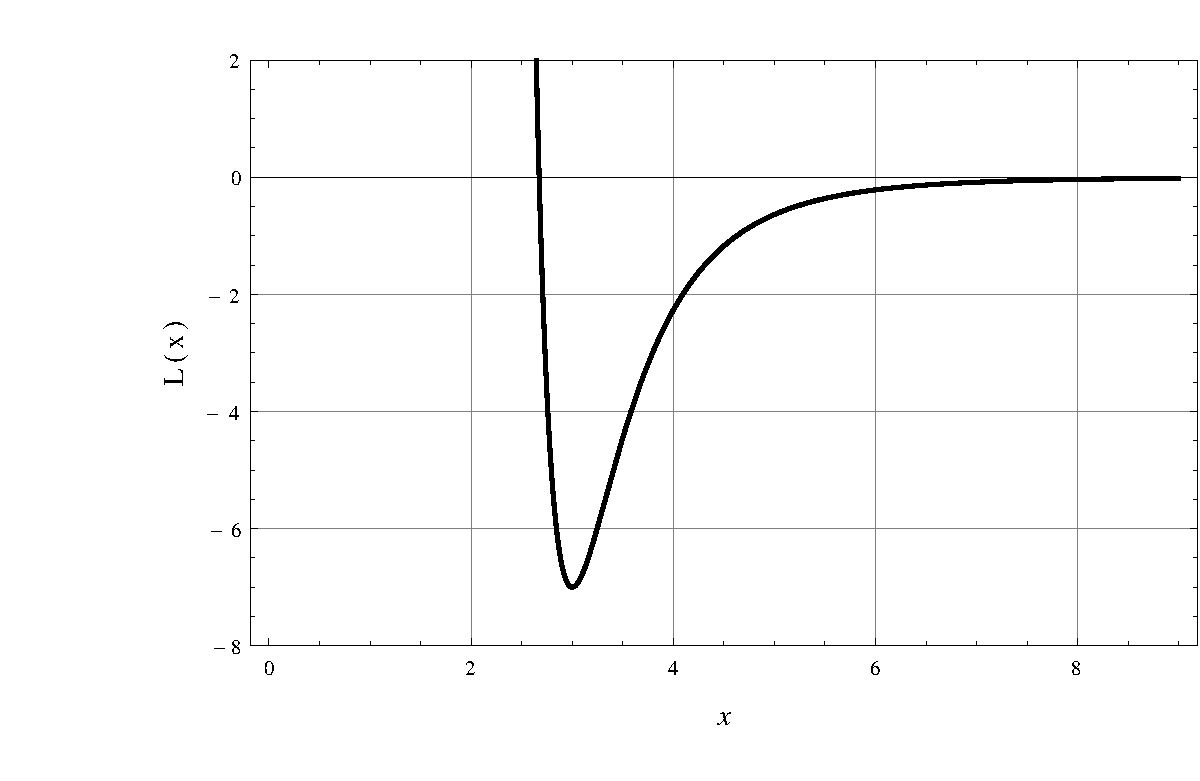
\includegraphics[width=0.5\linewidth]{./figures/LJPlots/LJ3_7.pdf}
    }
    \subfloat[][]{
	\label{fig:LJPlot2_4}
	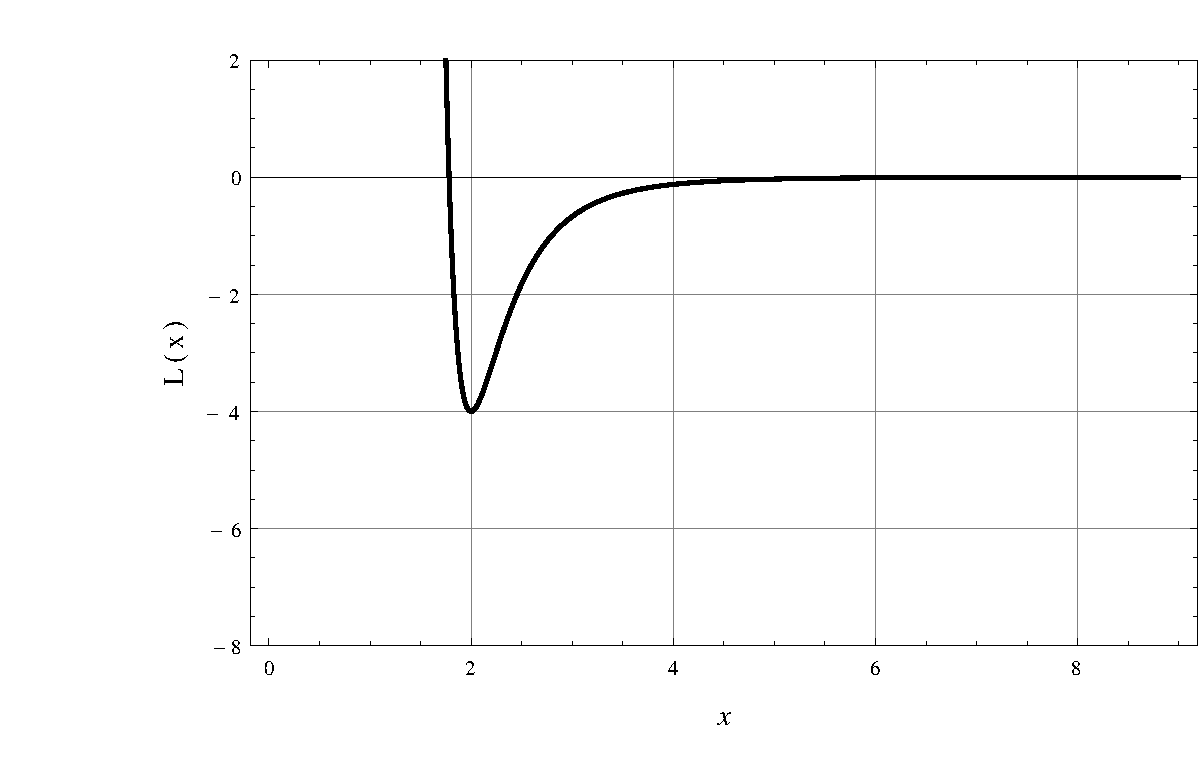
\includegraphics[width=0.5\linewidth]{./figures/LJPlots/LJ2_4.pdf}
    }\\

       \caption[Lennard-Jones Potential]{Plot of the Lennard-Jones potential for two different
	   parameter set. $r_m$ defines the position of the minimum and $\epsilon$ its depth.
    \subref{fig:LJPlot3_7} $r_m=2.0$ and $\epsilon=4.0$
    \subref{fig:LJPlot2_4} $r_m=3.0$ and $\epsilon=7.0$
    \label{fig:LJPlots}
    }

\end{figure}



\section{Taylor expansion} % (fold)
\label{sec:Non-Grid based methods}
From an algorithmic point of view it is of course desirable to have a set of closed form formulas for the the Morse parameters rather than having
to solve a large and possibly non-linear system of equations in every step of the algorithm. Thus, we first look if there is a straightforward way to
calculate the Morse potential parameters from locally available information about our target potential, that is the value of its derivatives.

\subsection{Coefficients of Taylor expansion} % (fold)
\label{sub:Coefficients of Taylor expansion}
To determine the three free parameters $x_0, V_0$ and $\beta$ we need three independent equations. We thus expand the Morse potential $M(x)$ to second
order which yields:
\begin{align}
	\begin{split}
    M(x)=&-2V_0e^{-\beta(q-x_0)}+V_0e^{-2(q-x_0)})\\
    &+2\beta V_0(e^{-\beta(q-x_0)}+e^{-2(q-x_0)})(x-q)\\
    &-\beta^2V_0(e^{-\beta(q-x_0)}+2V_0\beta^2e^{-2(q-x_0)})(x-q)^2+\bigO{(x-q)^3}
    \end{split}
\end{align}
Assuming that target potential $V(x)$ is at least $\mathcal{C}^2(\mathbb{R})$ we can compare coefficients and obtain the following non-linear
system:
\begin{align}
    \label{eq:TaylorParamsOrig}
    \begin{split}
    -2V_0e^{-\beta(q-x_0)}+V_0e^{-2\beta(q-x_0)}&=V(q):=P_1\\
    +2\beta V_0 e^{-\beta(q-x_0)}-2V_0\beta e^{-2\beta(q-x_0)}&=V'(q):=P_2\\
    -\beta^2V_0 e^{-\beta(q-x_0)}+2V_0\beta^2 e^{-2\beta(q-x_0)}&=\frac{V''(q)}{2}:=P_3
    \end{split}
\end{align}
With the substitution $A:=e^{-\beta(q-x_0)}$, this simplifies to the following system
of quadratic equations:
\begin{align}
    \begin{split}
	V_0(-2A+A^2)&=P_1\\
	2\beta V_0(A-A^2)&=P_2\\
	2\beta^2 V_0(-A+2A^2)&=P_3
    \end{split}
\end{align}
leading to the two solutions
\begin{align}
\beta&=\frac{-3P_2^2+\sqrt{9P_2^4-8P_3P_2^2P_1}}{4P_2P_1}\\
V_0^{(1,2)}&=\frac{\pm3P_2^4\pm8P_3^2P_1^2(\mp12P_3P_1\sqrt{9P_2^4-8P_3P_2^2P_1})}{\pm8P_3(P_2^2-P_3P_1)}\\
A^{(1,2)}&=\frac{\pm5P_2\mp4P_3P_1+\sqrt{P_2^2(9-P_2^2-8P_3P_1)}}{\pm4P_2^2-4P_3P_1}
\end{align}
which can then be subsequently solved for $x_0$.\\

Due to the quadratic nature of these equations,
we obtain two solutions, corresponding to the exact local expansion we are looking for and
a version that is mirrored either in $x$ or $y$-direction. Hence, for a general algorithm, 
additional steps must be employed to identify the correct one. Fits can be see in the following figure \ref{fig:MorseFitsTaylor}.


%Due to the non-linearity we cannot obtain an explicit expression for our parameters. Nevertheless, it would be possible to recast these equations as
%a root-finding problem and solve it numerically using Newton iteration for instance. However, for an arbitrary potential it is not clear whether
%a unique, physical solution exists and furthermore if the algorithm will converge to it. \\
%
%Another possibility is to simplify the expression by expanding the Morse potential around its minimum:
%\begin{equation}
%    \label{eq:MorseTaylor2nd}
%    -V_0+\beta^2V_0(x-x_0)^2+\bigO{(x-x_0)^3}
%\end{equation}
%By that choice we implicitly fix the former free parameter $x_0$ to the current mean location $q$ of the wave packet we wish to propagate.
%In that can case we can also find an easy expression for the coefficients of the Taylor expansion:
%\begin{equation}
%    \label{eq:MorseTaylorCoeff}
%    \frac{(-2+2^n)(-\beta)^nV_0}{n!},\quad n\in\mathbb{N}
%\end{equation}
%
%Comparing coefficients again with the expansion of the potential $V(x)$ around $q=x_0$ leads to the following simple set of equations:
%\begin{align}
%    \label{eq:TaylorParams}
%    \begin{split}
%	-V_0	    &=  V(x_0)\\
%        0	    &=  V'(x_0)\\
%	\beta^2V_0  &=	\frac{V''(x_0)}{2}
%    \end{split}
%\end{align}
%From that we can indeed easily derive expressions for our parameters $\beta$ and $V_0$:
%\begin{equation}
%    V_0=-V(x_0),\qquad \beta=\sqrt{\frac{-V''(x_0)}{2V(x_0)}}
%\end{equation}
%Naturally, the second equation in \eqref{eq:TaylorParams} came about by choosing $q=x_0$ to be the minimum of the Morse potential.
%This is problematic since it basically demands that the potential $V(x)$ is extremal in $x_0$ as well, which is of course not necessarily the case.
%Even though we only need a locally good Morse-like approximation to the potential we can see in the following figures \ref{fig:MorseFitsTaylor} that if the extremality
%condition is violated, the Morse approximation becomes useless. 
\begin{figure}[h!]
    \centering
%     \subfloat[][]{
%	\label{fig:Taylor090}
%	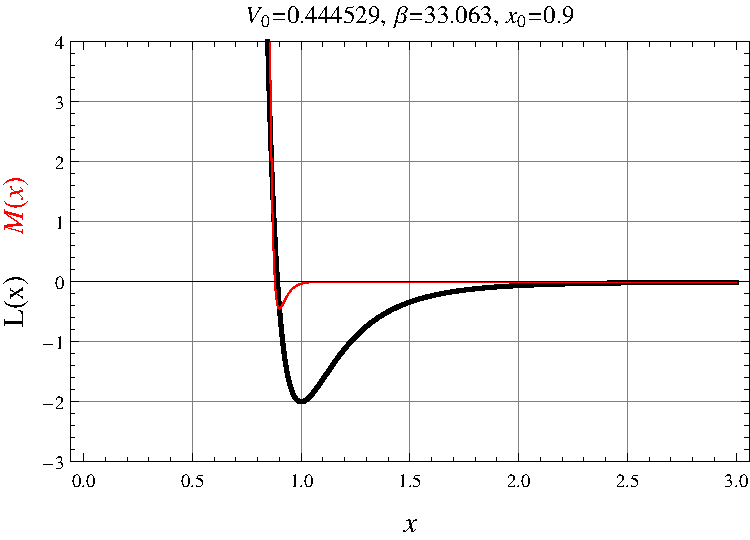
\includegraphics[width=0.5\linewidth]{./figures/MorseFitsTaylor/Taylor090.pdf}
%    }
%    \subfloat[][]{
%	\label{fig:Taylor100}
%	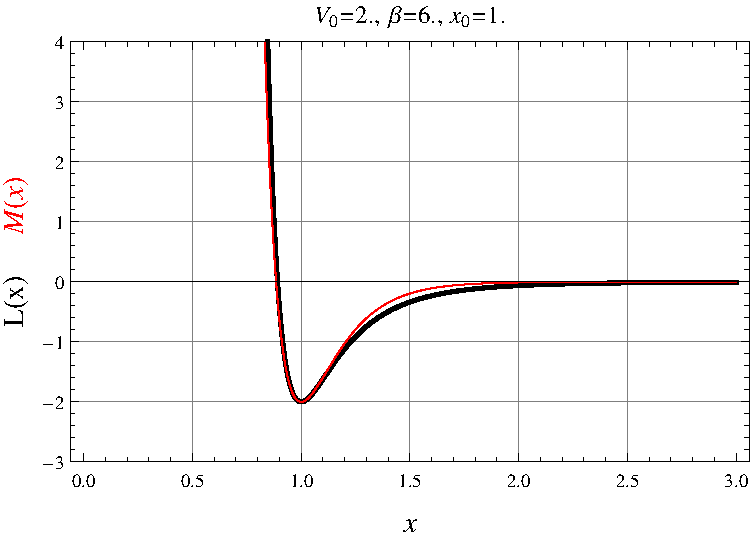
\includegraphics[width=0.5\linewidth]{./figures/MorseFitsTaylor/Taylor100.pdf}
%    }\\
%    \subfloat[][]{
%	\label{fig:Taylor105}
%	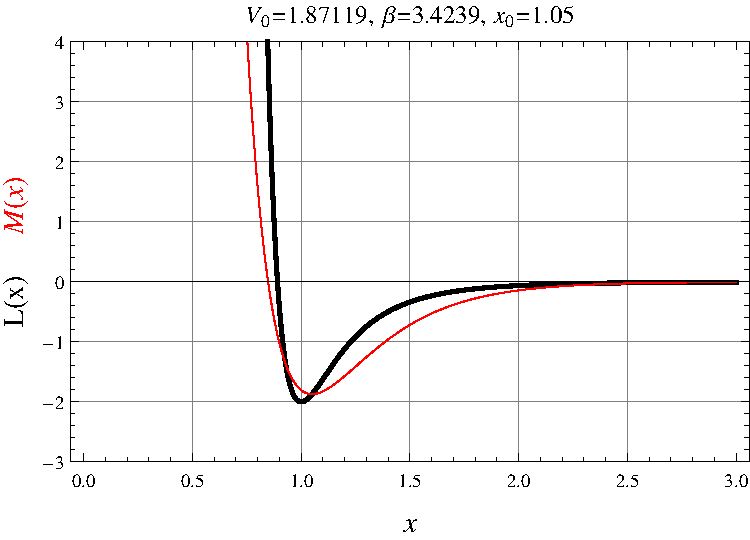
\includegraphics[width=0.5\linewidth]{./figures/MorseFitsTaylor/Taylor105.pdf}
%    }
%    \subfloat[][]{
%	\label{fig:Taylor110}
%	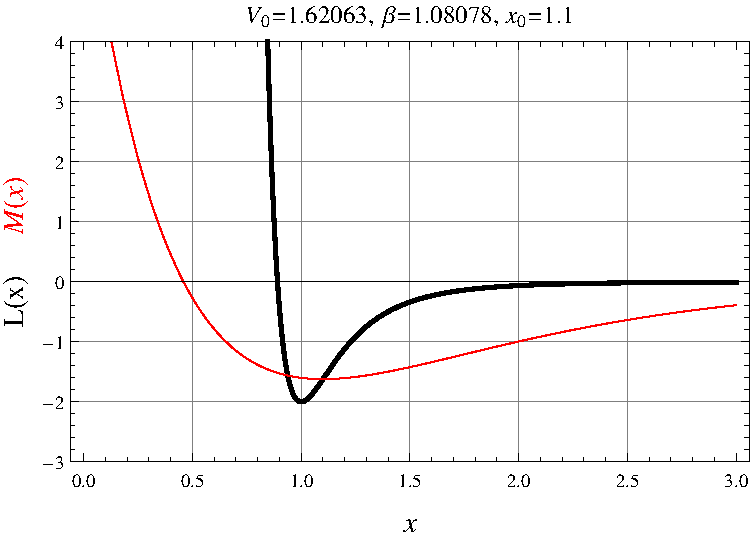
\includegraphics[width=0.5\linewidth]{./figures/MorseFitsTaylor/Taylor110.pdf}
%    }
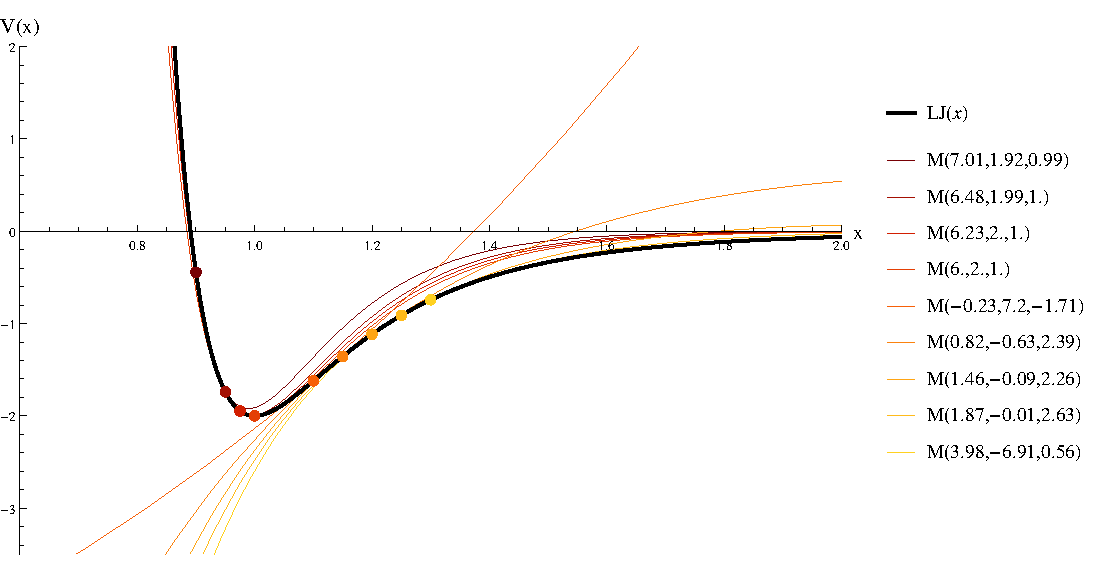
\includegraphics[width=1.2\linewidth]{./figures/MorseFitsTaylor/taylorfitsAll.pdf}
    \\

       \caption[Fits using Taylor series coefficient equations]{\textbf{Fits using Taylor series coefficient equations}:
	In the plots we see the results of fitting the Morse potential to a Lennard-Jones potential with $r_m=1.0$ and $\epsilon=2.0$.
	    \label{fig:MorseFitsTaylor}
    }

\end{figure}

% subsection Coefficients of Taylor expansion (end)

% section Least Square methods

\section{Least Square methods} % (fold)
\label{sec:LeastSquareMethods}
The basic problem of the previous approach is that we only use the information available at the point $q$ by a comparison to a polynomial approximation.
To obtain better results one has to explicitly minimize the error in the region of interest around $q$ which naturally leads to a least squares 
approach. For a given potential $V(x)$ one tries to find  Morse parameters $x_0, V_0$ and $\beta$ such that

\begin{equation}
    \label{eq:lstsqprob}
    S(x_0, V_0, \beta)=\sum_{i=1}^N[V(x_i)-M(x_i,x_0,V_0, \beta)]^2 
\end{equation}
becomes minimal. For simplicity, the sample points $\lbrace x_i\rbrace_{i=1}^N$ are chosen equidistant within a $\delta$-neighborhood around 
the current mean wave packet position $q$ while the current width wave packet parameter $Q$ might be a good indicator for choosing the size
of $\delta$. \\
Also the distribution of the sample points within that interval might be chosen more concentrated in the center of the interval or adapted
to other components of a potential Morse packet time-stepping algorithm. Depending on the quality of the fit one could already sample
the quadrature nodes for the Galerkin approximation in the last step of the algorithm.\\

For the test with the Lennard-Jones potential the Python routines \texttt{curve\_fit} and \texttt{leastsq} from the \texttt{scipy.optimize}
package were used. \\
% section Grid based methods (end)


\subsection{\texttt{curve\_fit}} % (fold)
\label{sub:curve_fit}
The function \texttt{curve\_fit} is actually just  a wrapper for \texttt{leastsq} but in the latter case one can also provide an analytical Jacobian while
\texttt{curve\_fit}, by default, estimates it. The underlying FORTRAN library \textbf{MINPACK} implements the Levenberg-Marquardt algorithm (LMA),
also known as damped least-squares method to solve the least squares problem \eqref{eq:lstsqprob}.\\
The results of these fits are shown in Figure \ref{fig:MorseFitsCurvefit}.

\begin{figure}[h!]
    \centering
%     \subfloat[][]{
%	\label{fig:CurveFit09}
%	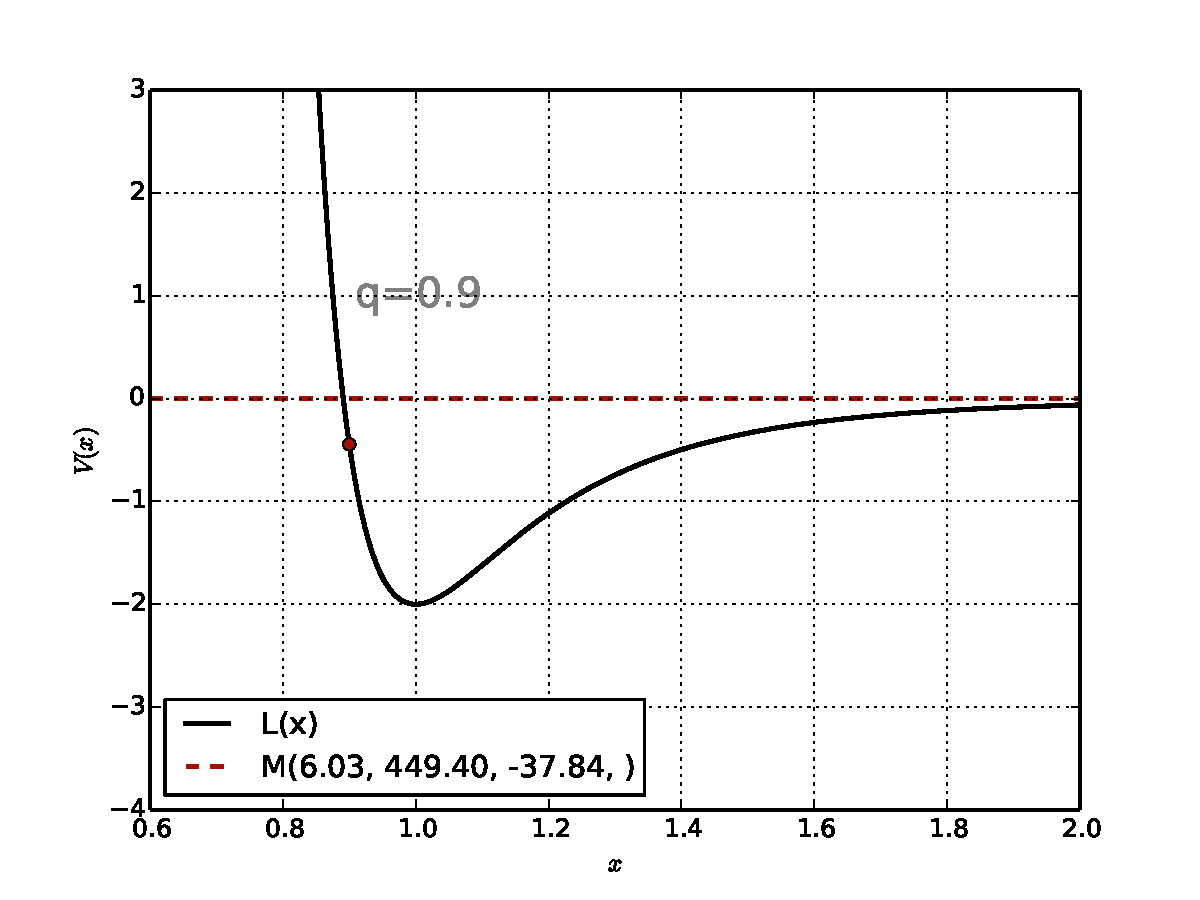
\includegraphics[width=0.5\linewidth]{./figures/MorseFitsCurvefit/curvefit09.pdf}
%    }
%    \subfloat[][]{
%	\label{fig:CurveFit095}
%	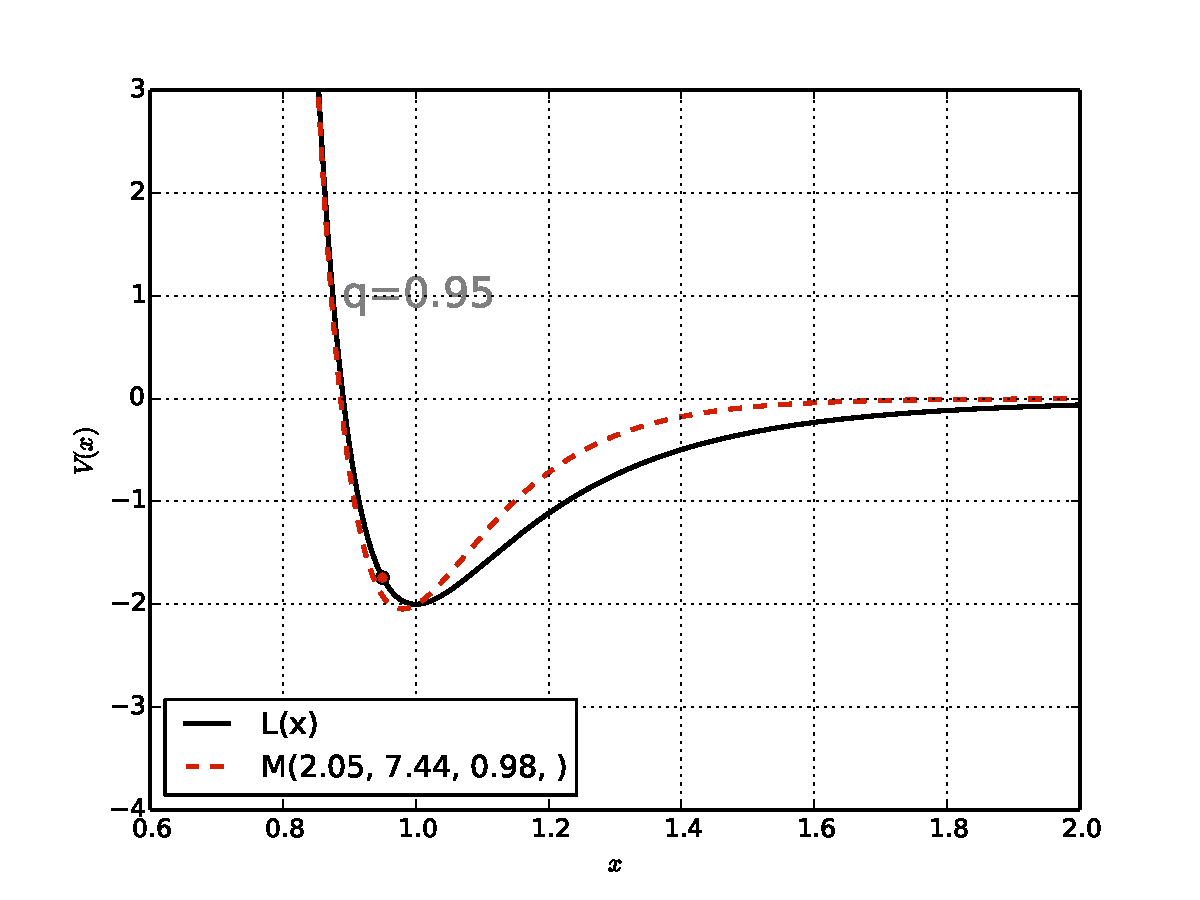
\includegraphics[width=0.5\linewidth]{./figures/MorseFitsCurvefit/curvefit095.pdf}
%    }\\
%    \subfloat[][]{
%	\label{fig:CurveFit0975}
%	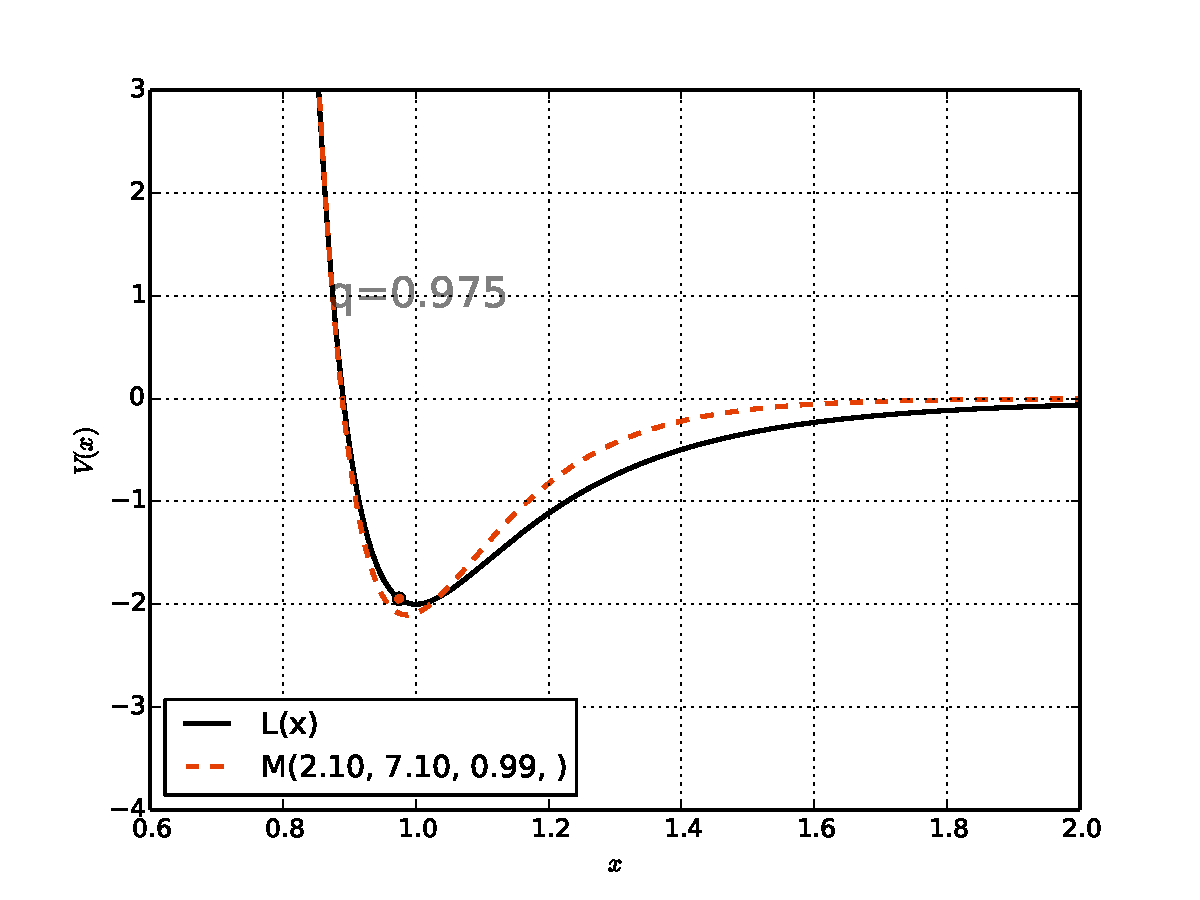
\includegraphics[width=0.5\linewidth]{./figures/MorseFitsCurvefit/curvefit0975.pdf}
%    }
%    \subfloat[][]{
%	\label{fig:CurveFit10}
%	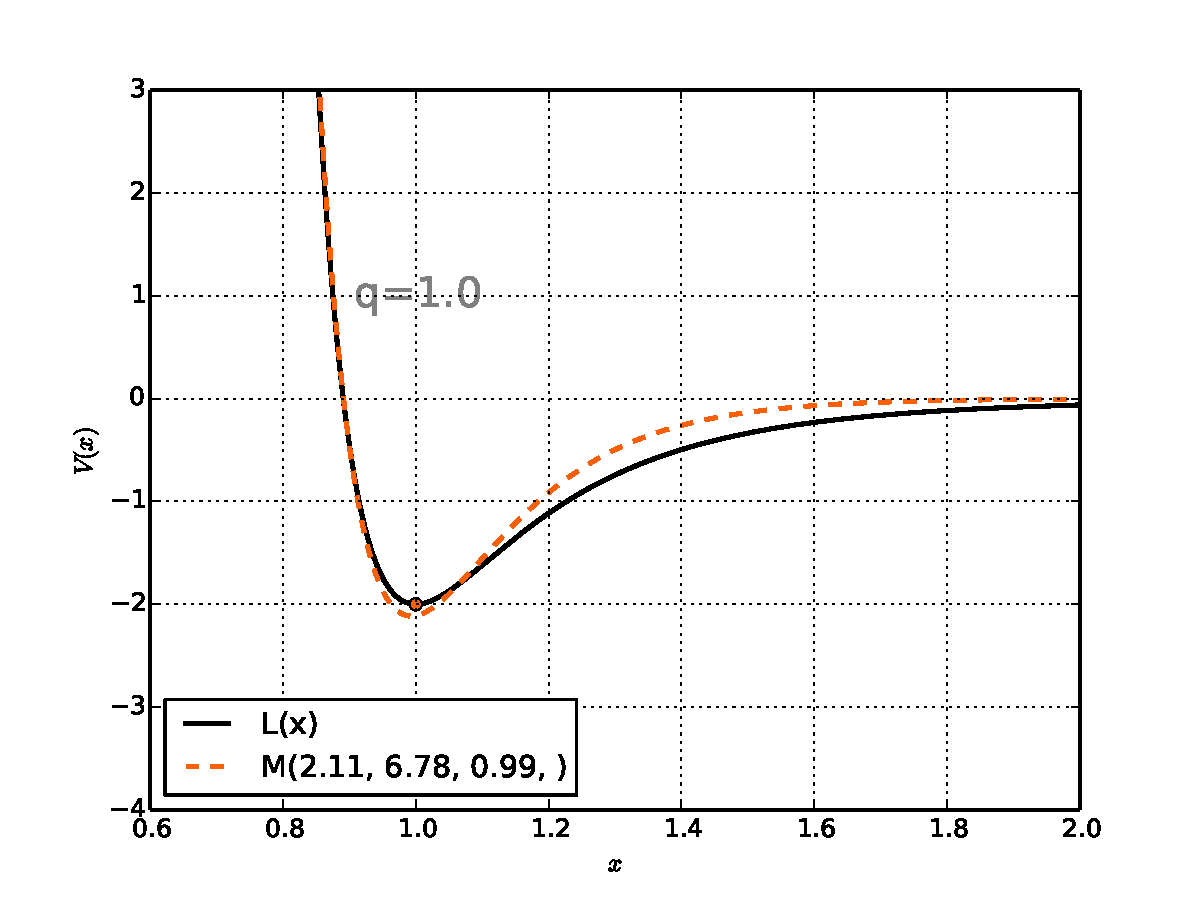
\includegraphics[width=0.5\linewidth]{./figures/MorseFitsCurvefit/curvefit10.pdf}
%    }
%    \\
%     \subfloat[][]{
%	\label{fig:CurveFit11}
%	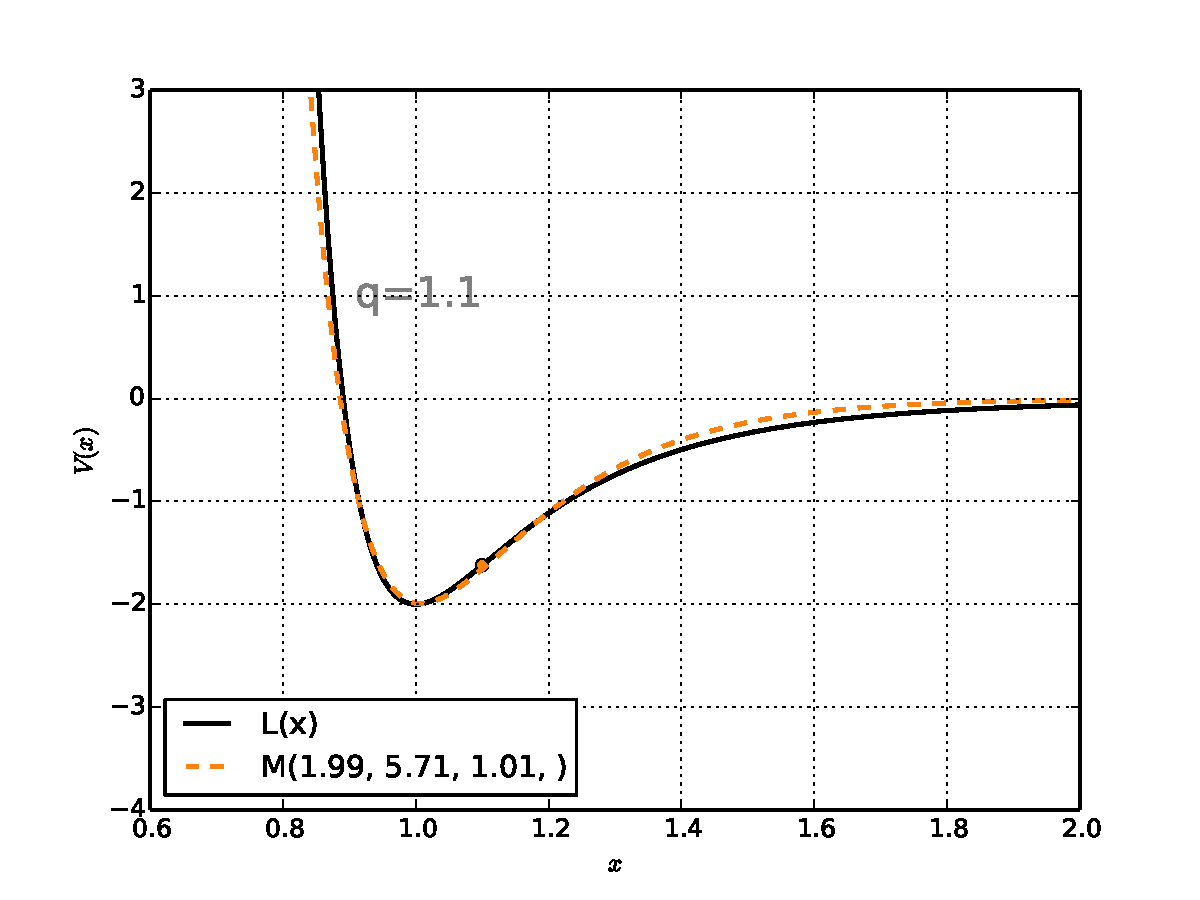
\includegraphics[width=0.5\linewidth]{./figures/MorseFitsCurvefit/curvefit11.pdf}
%    }
%    \subfloat[][]{
%	\label{fig:CurveFit115}
%	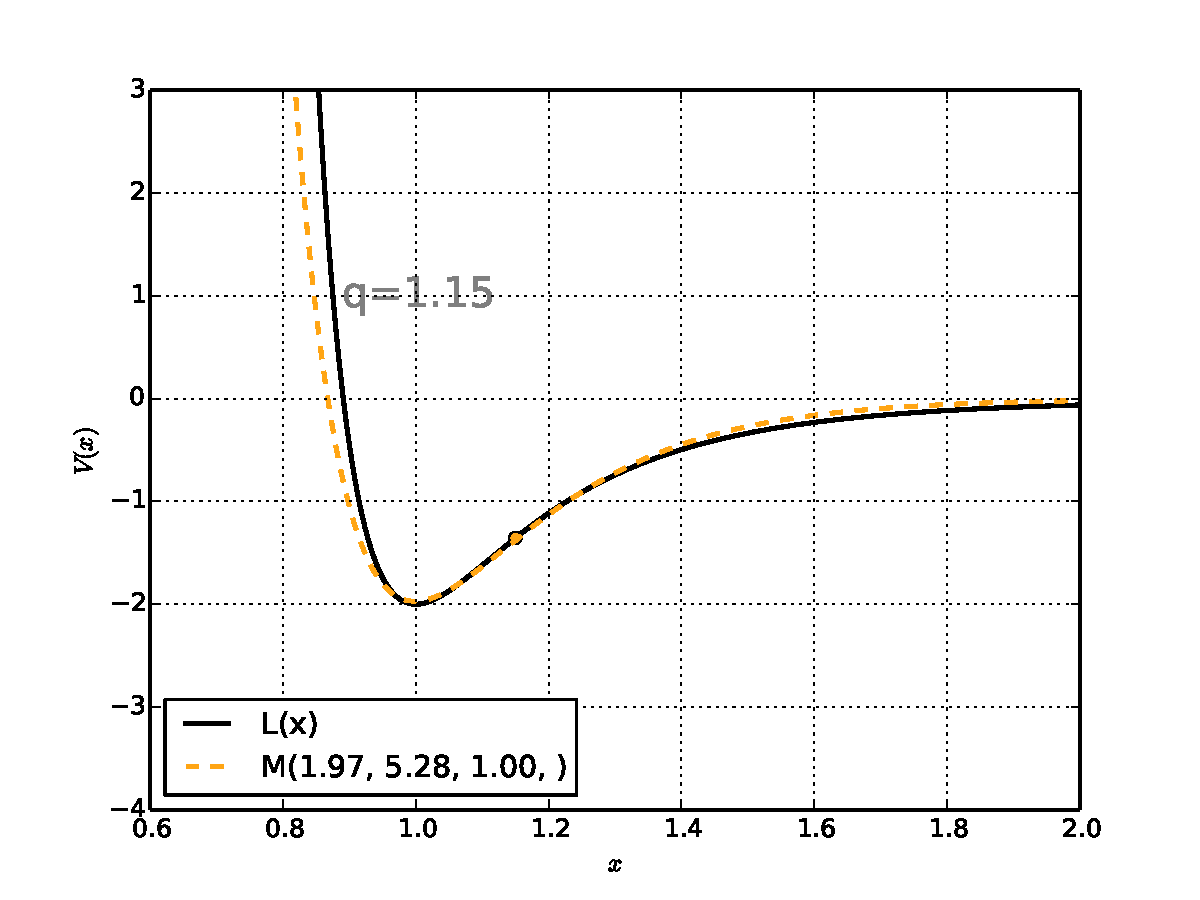
\includegraphics[width=0.5\linewidth]{./figures/MorseFitsCurvefit/curvefit115.pdf}
%    }\\
%    \subfloat[][]{
%	\label{fig:CurveFit12}
%	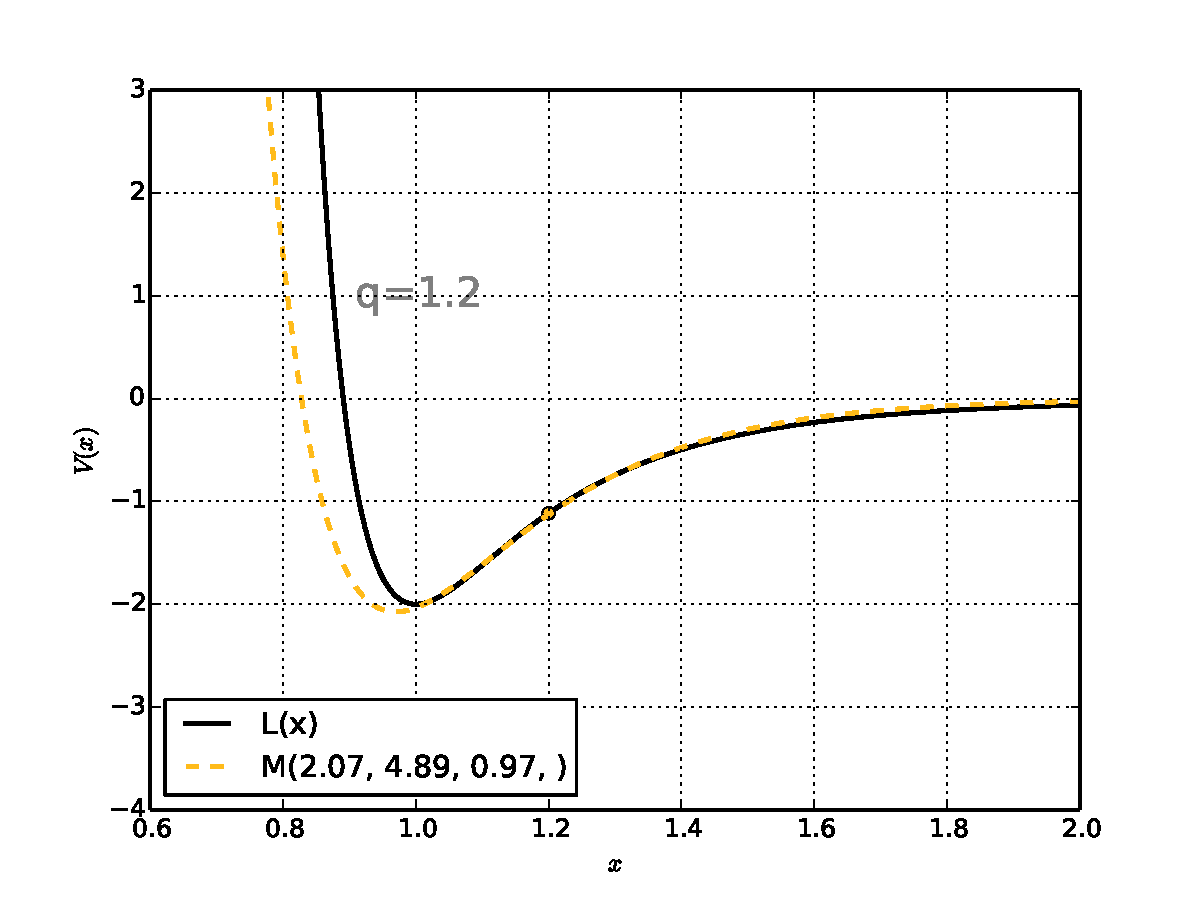
\includegraphics[width=0.5\linewidth]{./figures/MorseFitsCurvefit/curvefit12.pdf}
%    }
%    \subfloat[][]{
%	\label{fig:CurveFit125}
%	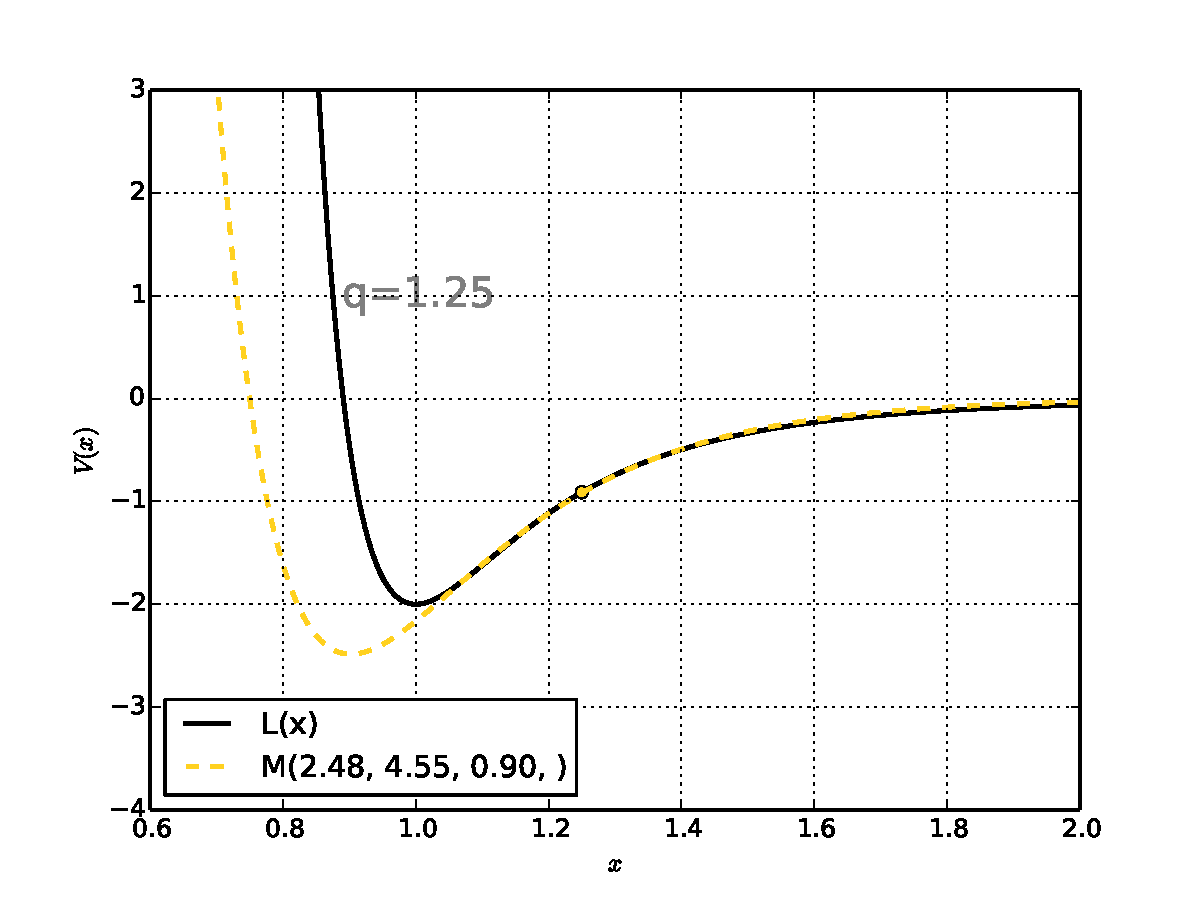
\includegraphics[width=0.5\linewidth]{./figures/MorseFitsCurvefit/curvefit125.pdf}
%    }
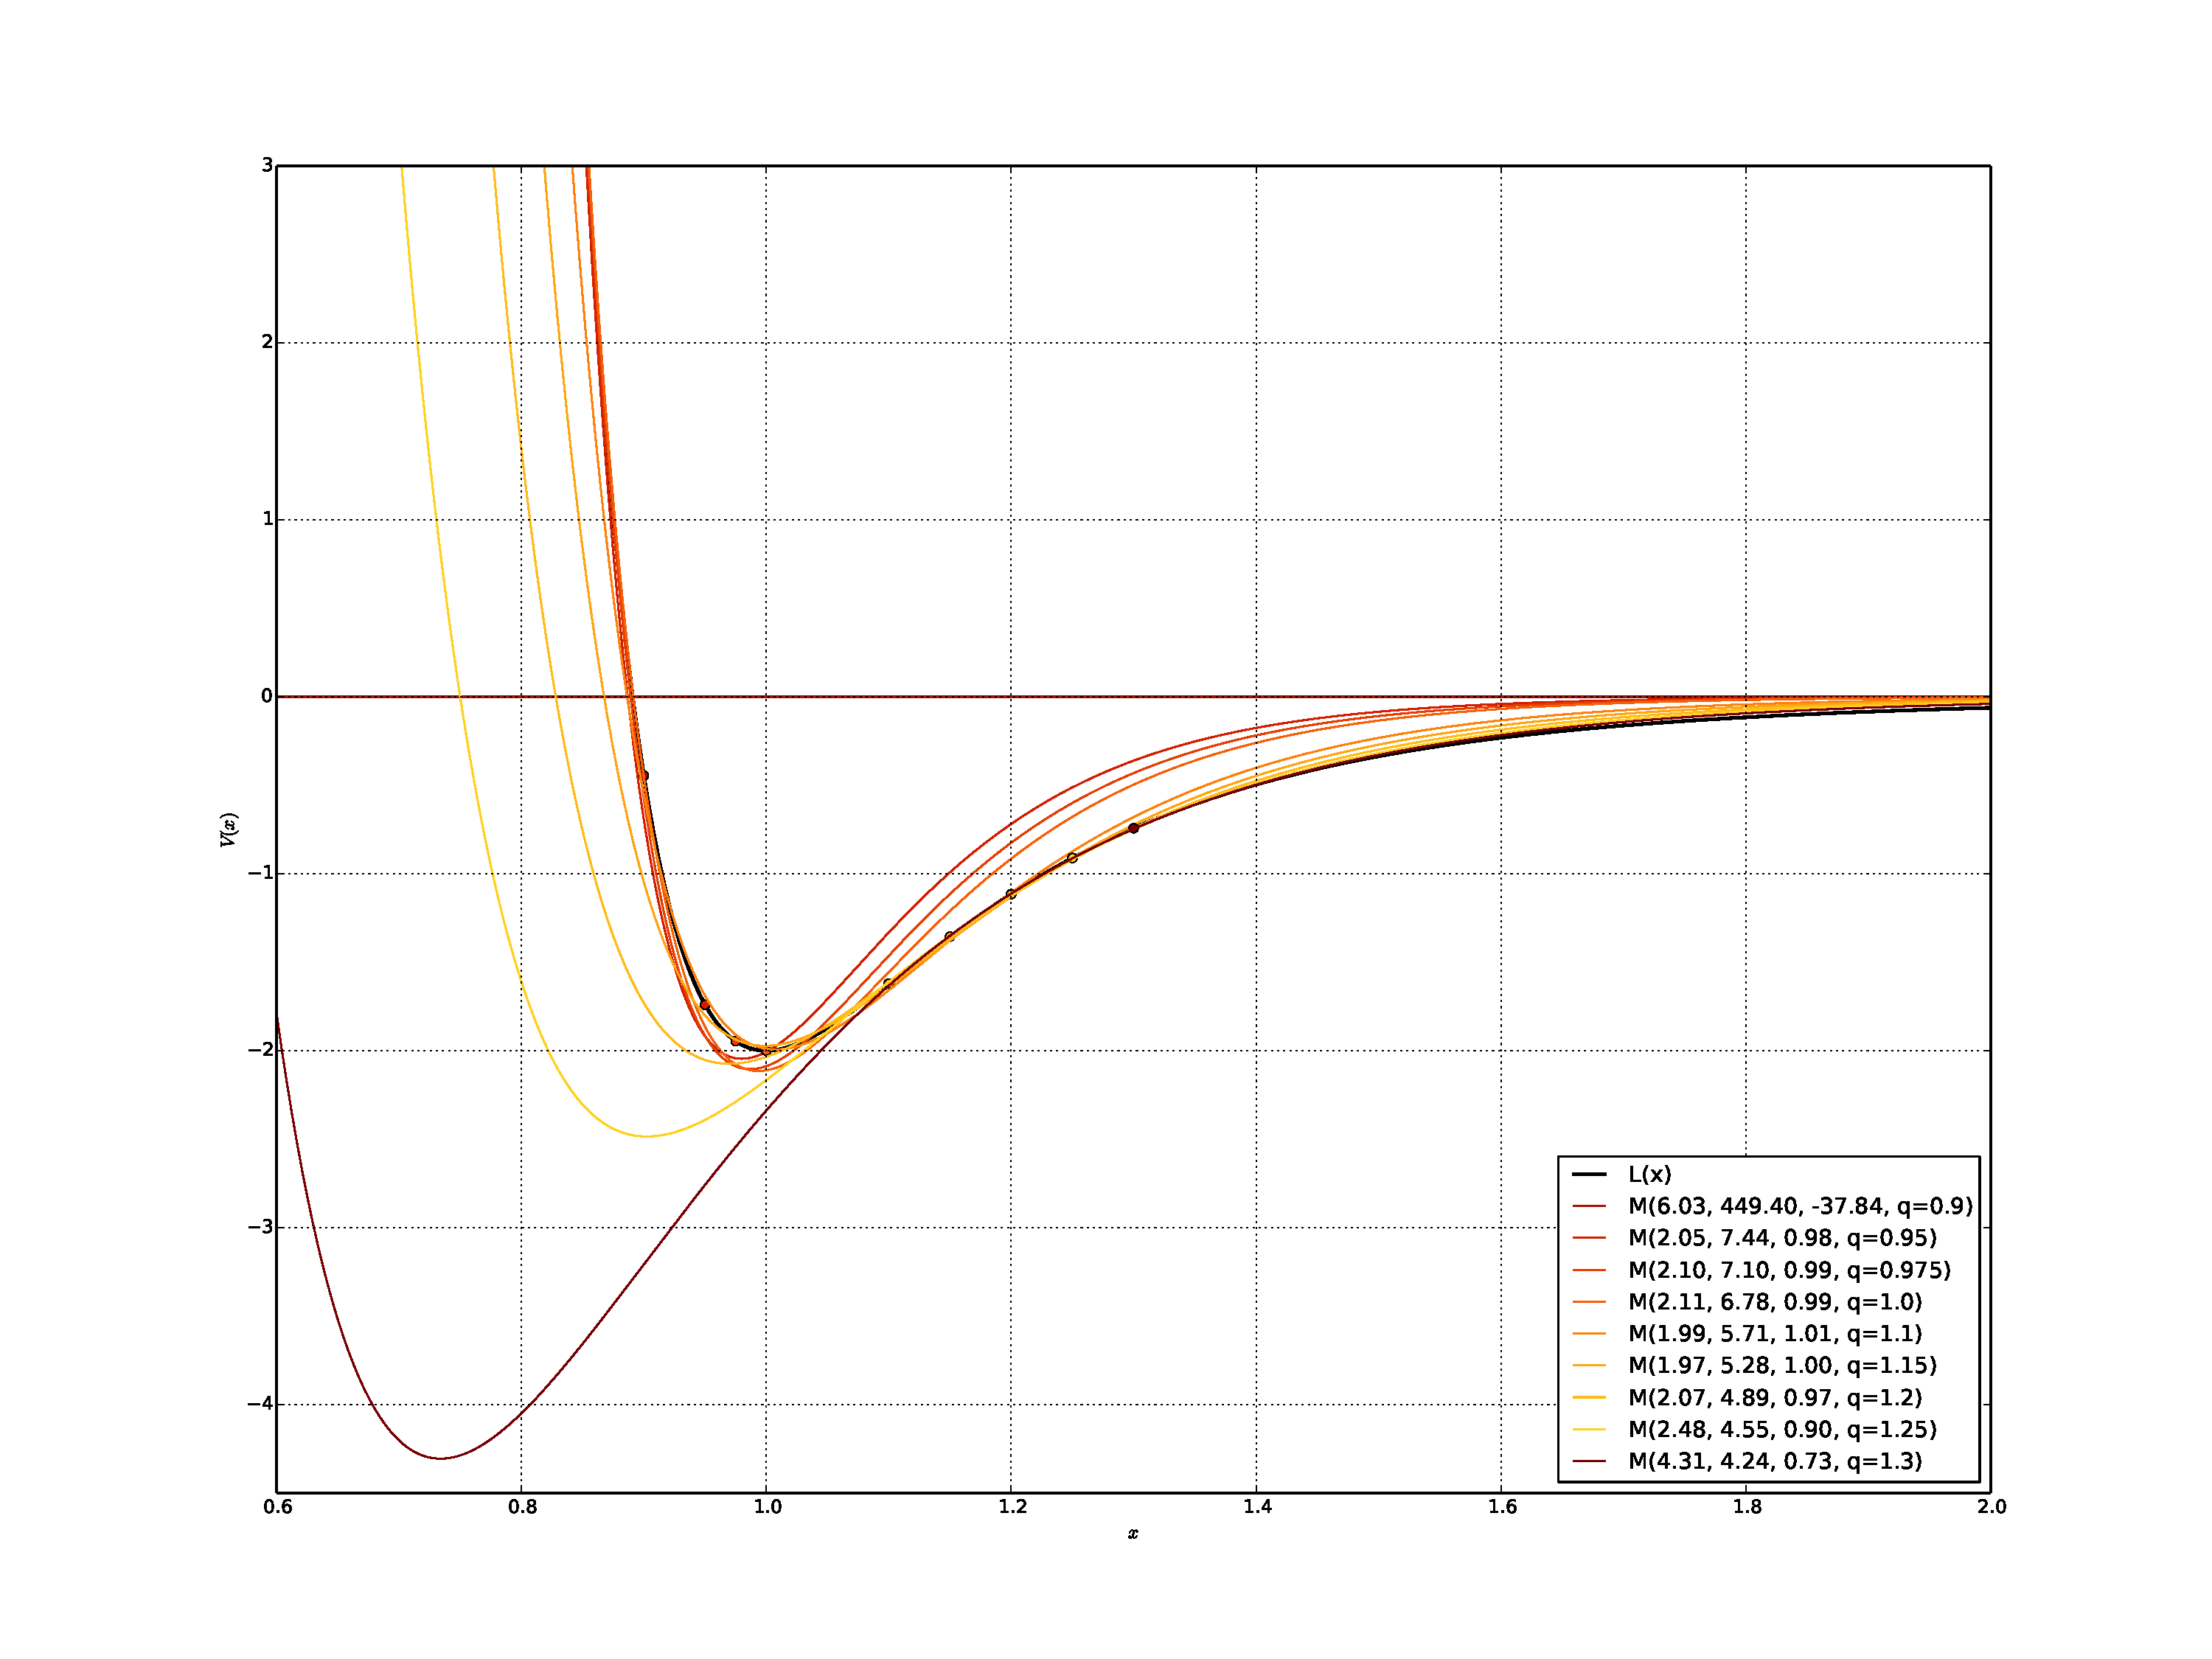
\includegraphics[width=1.2\linewidth]{./figures/MorseFitsCurvefit/curvefitAll.pdf}
    \\
%	\subfloat[][]{
%	\label{fig:CurveFit13}
%	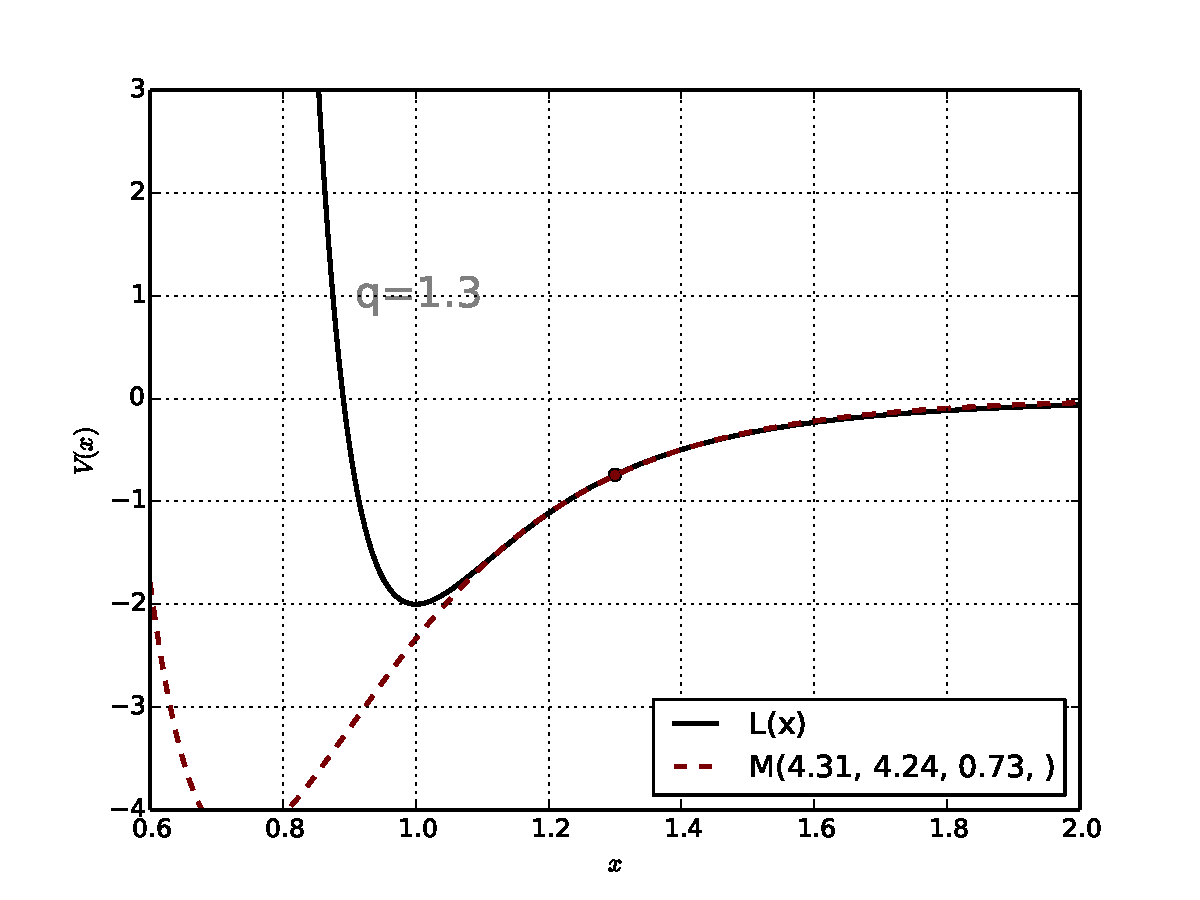
\includegraphics[width=0.5\linewidth]{./figures/MorseFitsCurvefit/curvefit13.pdf}
%    }
       \caption[\texttt{curve\_fit} fits to the Morse potential]{
	\texttt{curve\_fit} fits to the Morse potential
    \label{fig:MorseFitsCurvefit}
    }

\end{figure}



%\begin{figure}[h!]
%	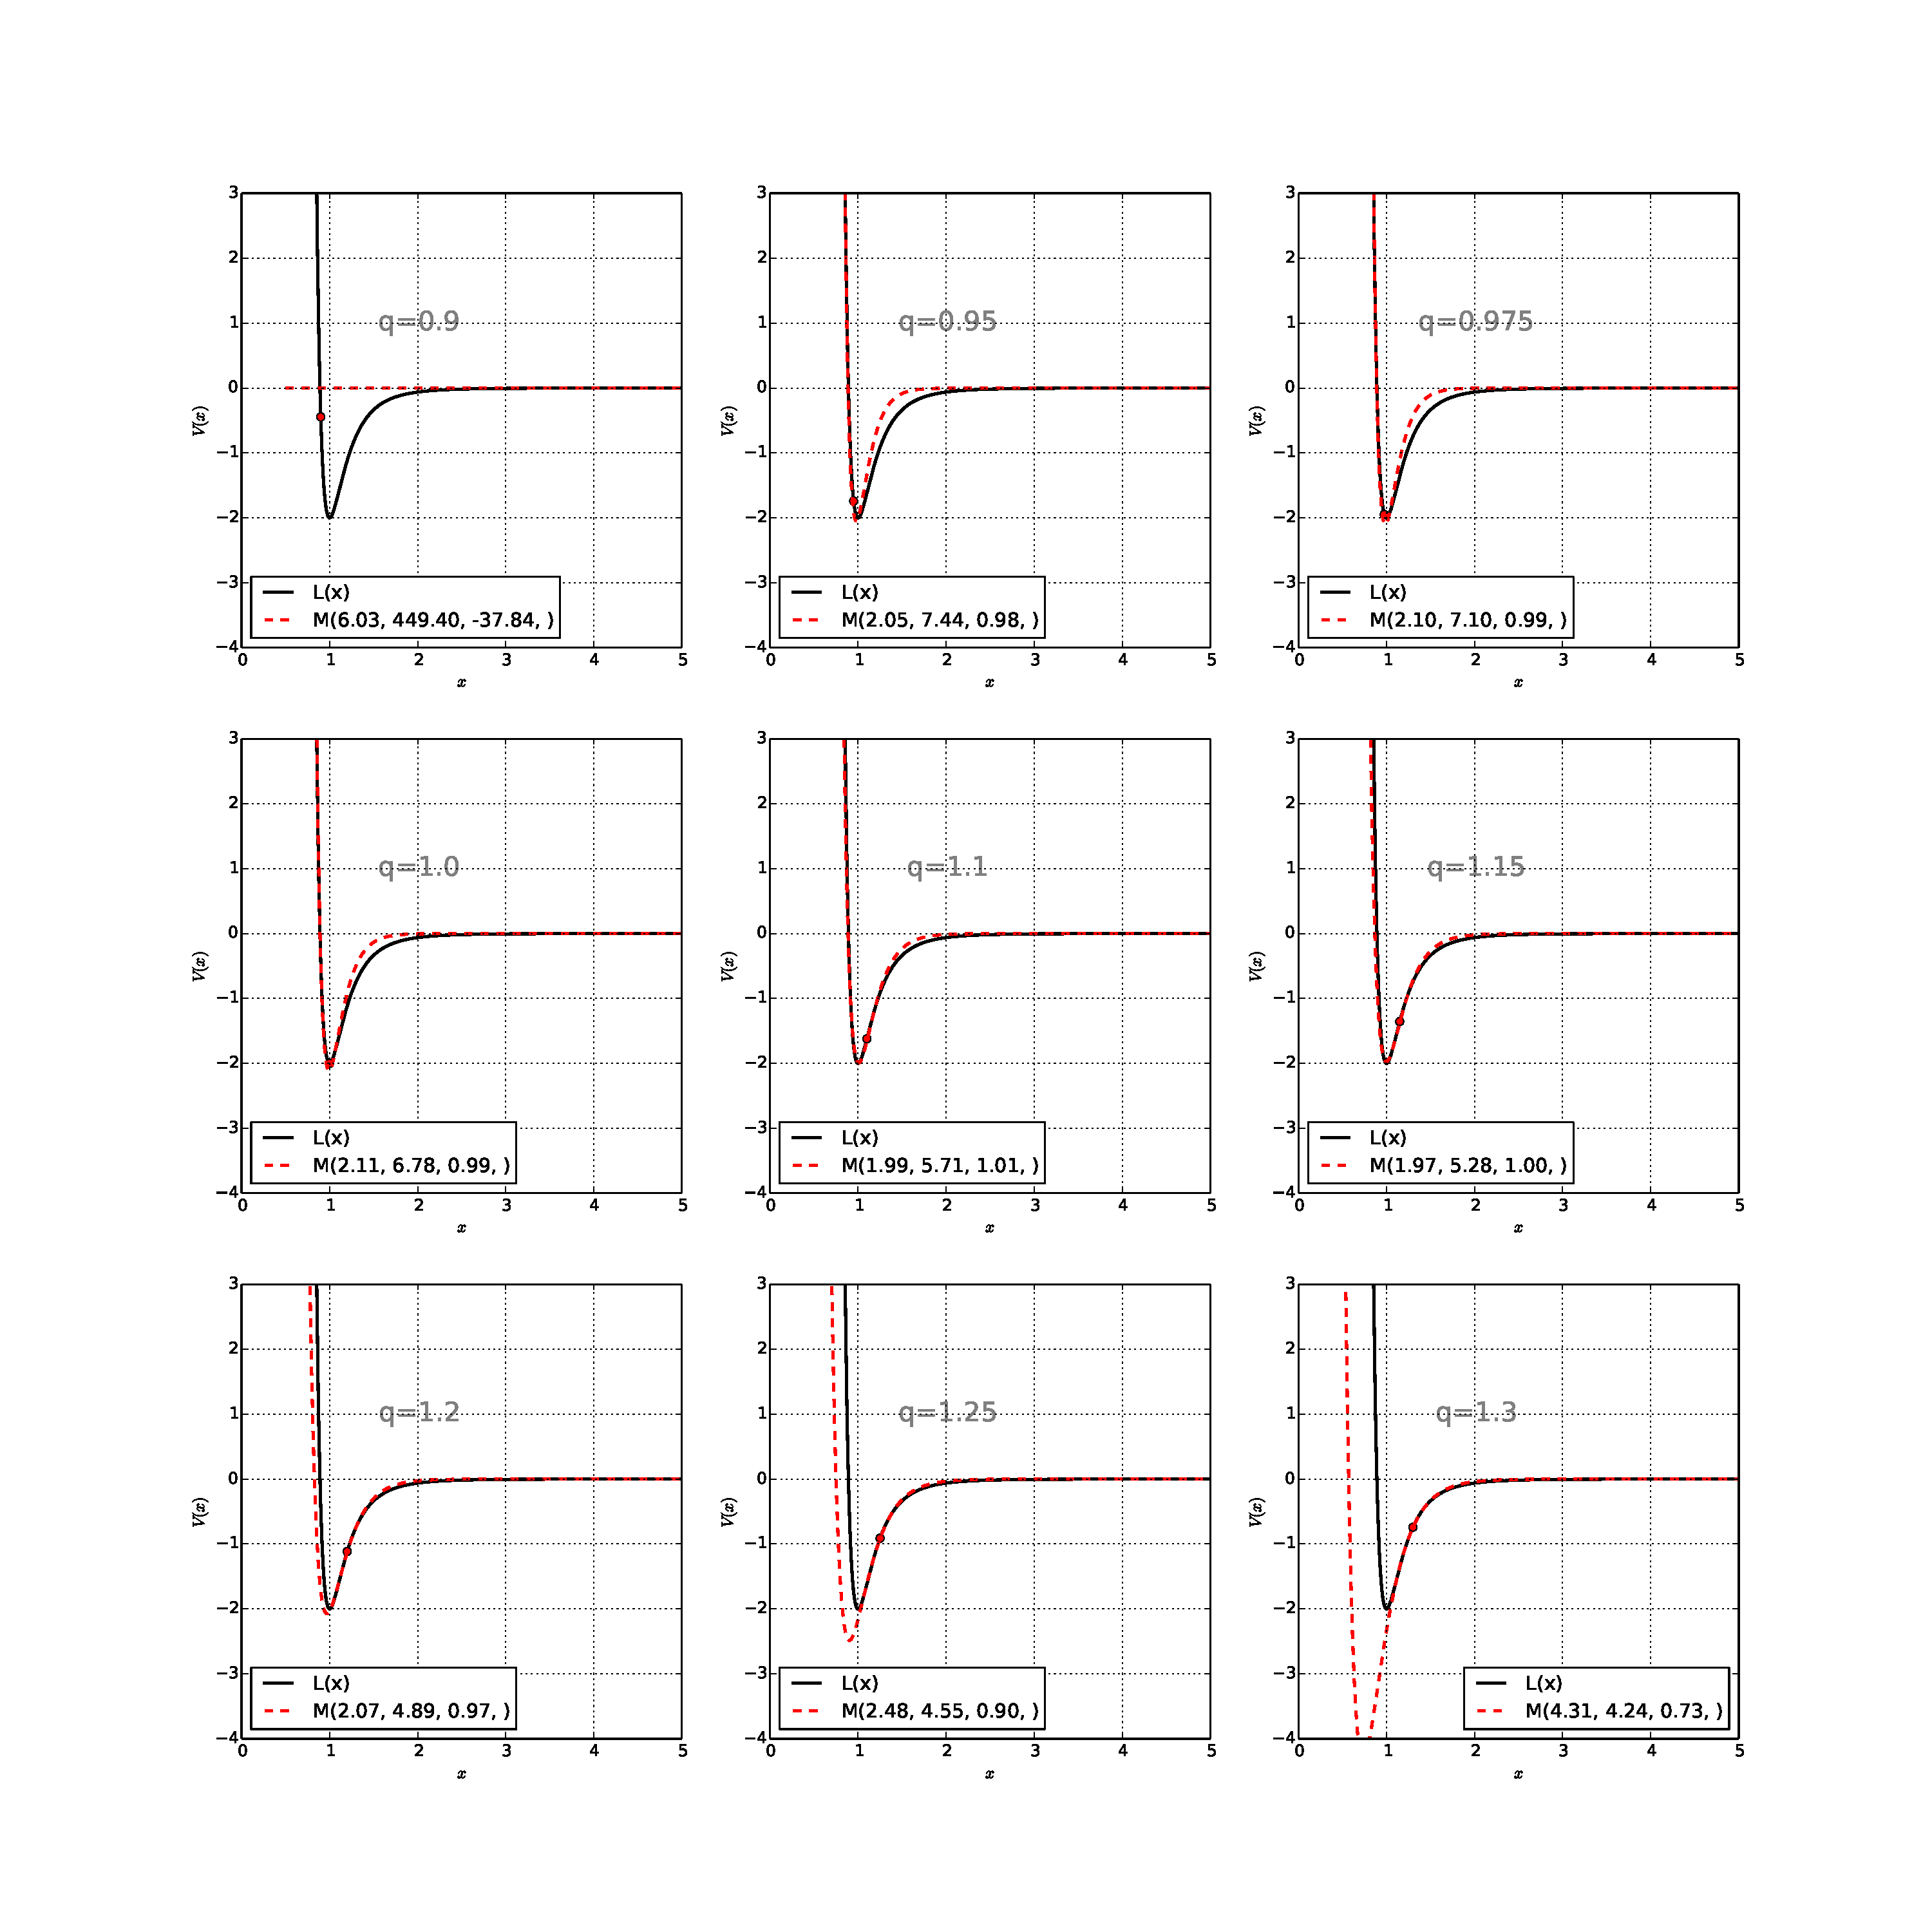
\includegraphics[width=1.0\linewidth]{./figures/MorseFitsCurvefit/fits_curvefit.pdf}
%	\caption[\texttt{curve\_fit} fits to the Morse potential]{
%	
%	    \label{fig:MorseFitsCurvefit}
%	}
%
%\end{figure}




% subsection curve_fit (end)

\subsection{\texttt{leastsq}}% (fold)
\label{subsec:leastsq}
As already said, the only difference to the previous algorithm is that we also provide an analytical Jacobian,
in our case given by
\begin{align}
    J_i=J(x_i)+
    \begin{pmatrix}
    	e^{-2\beta(x_i-x_0)}-2e^{-\beta(x_i-x_0)}\\
	-2 V_0 (x_i-x_0)(e^{-2\beta(x_i-x_0)}-2e^{-\beta(x_i-x_0)})\\
	2\beta(e^{\beta(x_i-x_0)}-2e^{-\beta(x_i-x_0)}
    \end{pmatrix}
\end{align}
% subsection leastsq (end)

\begin{figure}[h!]
    \centering
%     \subfloat[][]{
%	\label{fig:LeastSq09}
%	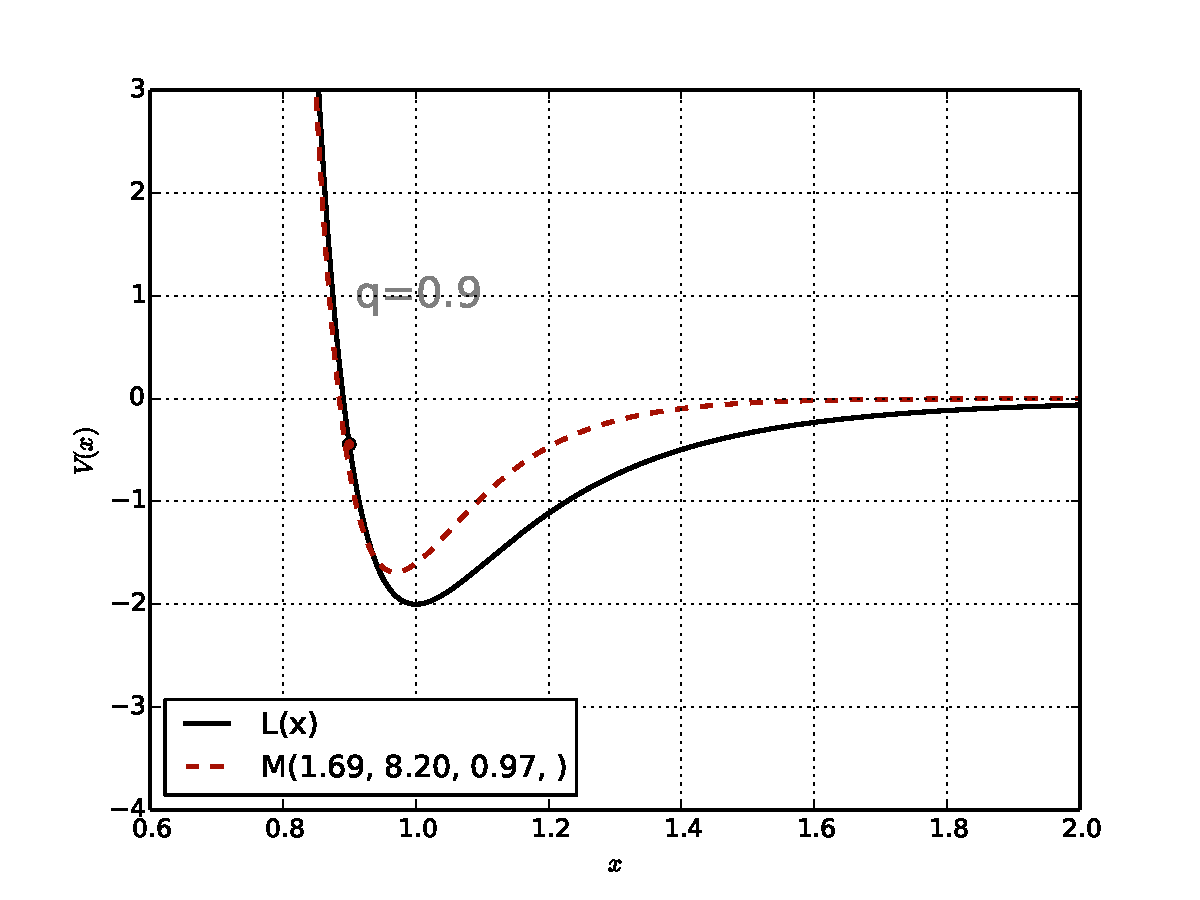
\includegraphics[width=0.5\linewidth]{./figures/MorseFitsLeastsq/leastsq09.pdf}
%    }
%    \subfloat[][]{
%	\label{fig:LeastSq095}
%	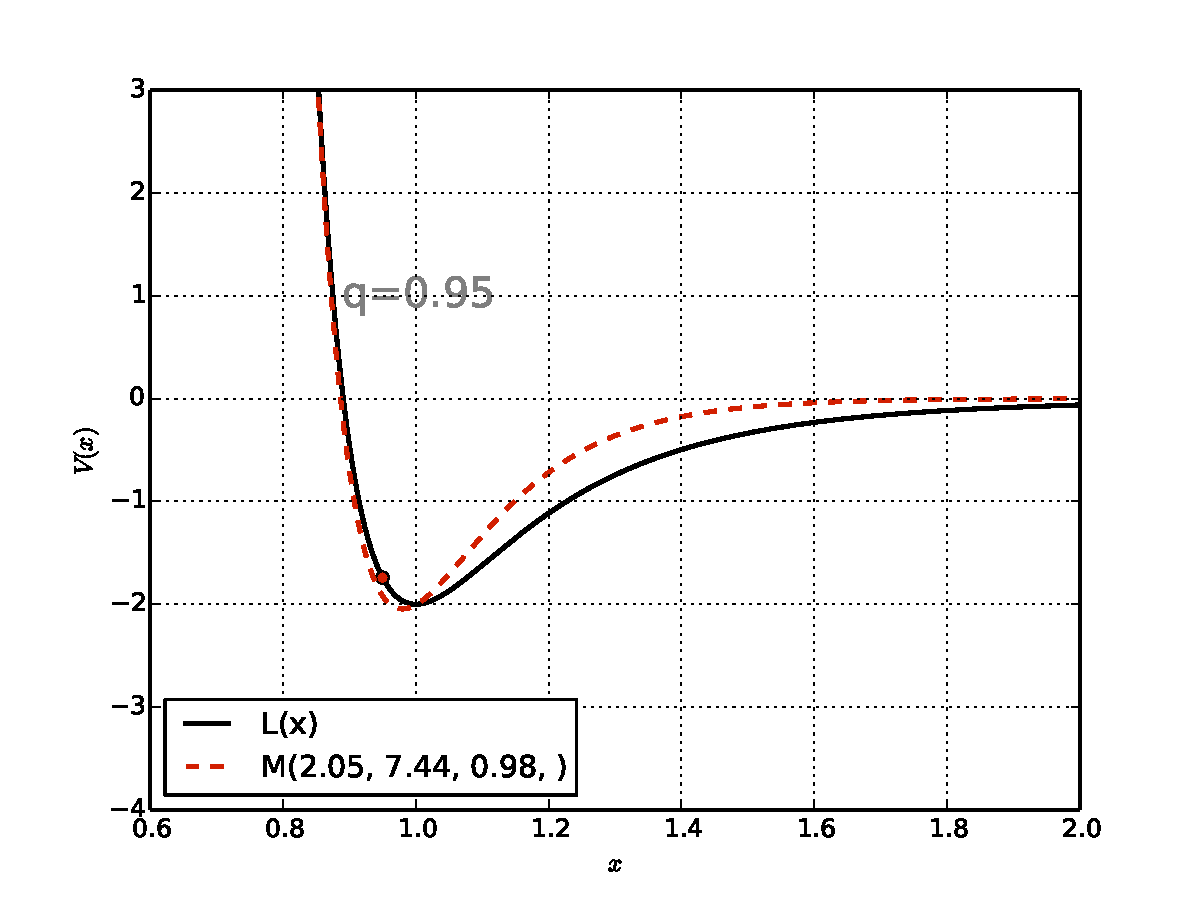
\includegraphics[width=0.5\linewidth]{./figures/MorseFitsLeastsq/leastsq095.pdf}
%    }\\
%    \subfloat[][]{
%	\label{fig:LeastSq0975}
%	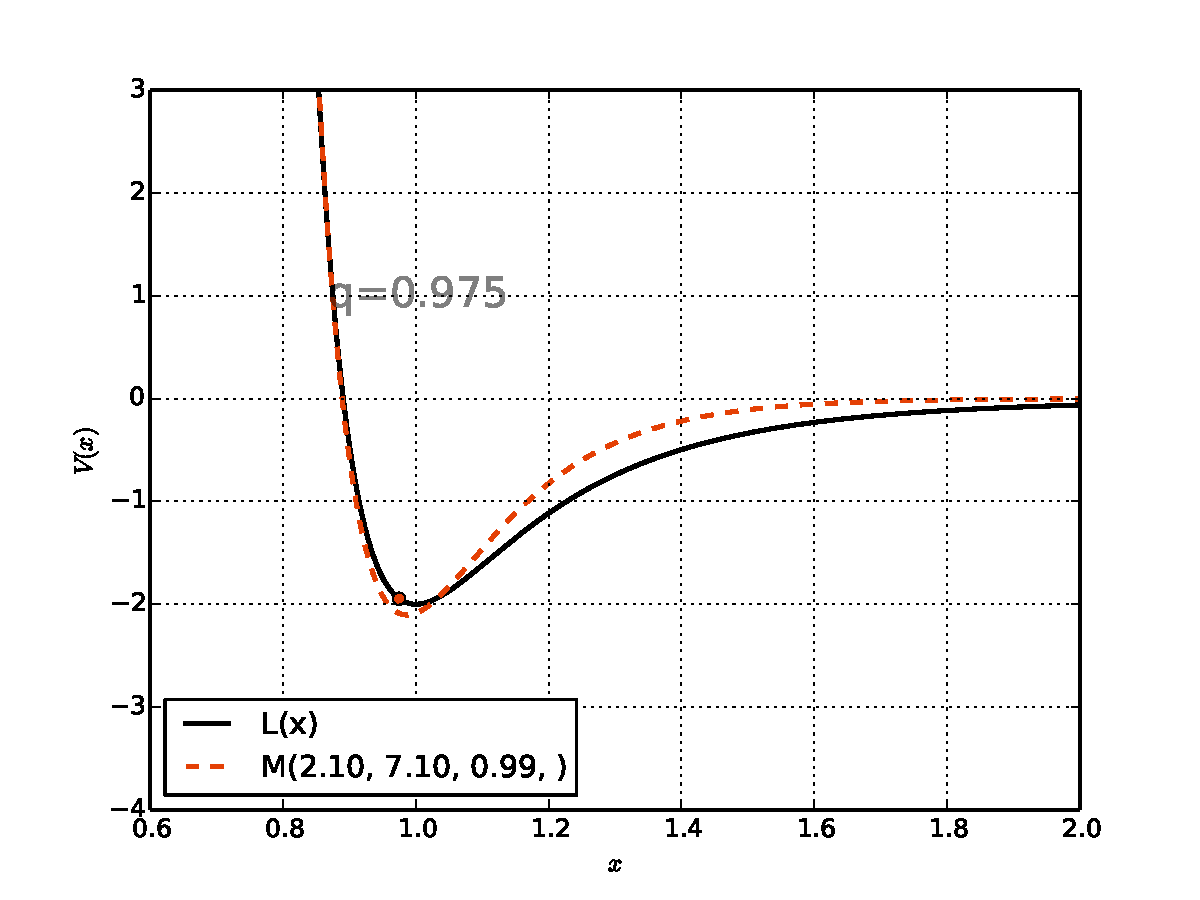
\includegraphics[width=0.5\linewidth]{./figures/MorseFitsLeastsq/leastsq0975.pdf}
%    }
%    \subfloat[][]{
%	\label{fig:LeastSq10}
%	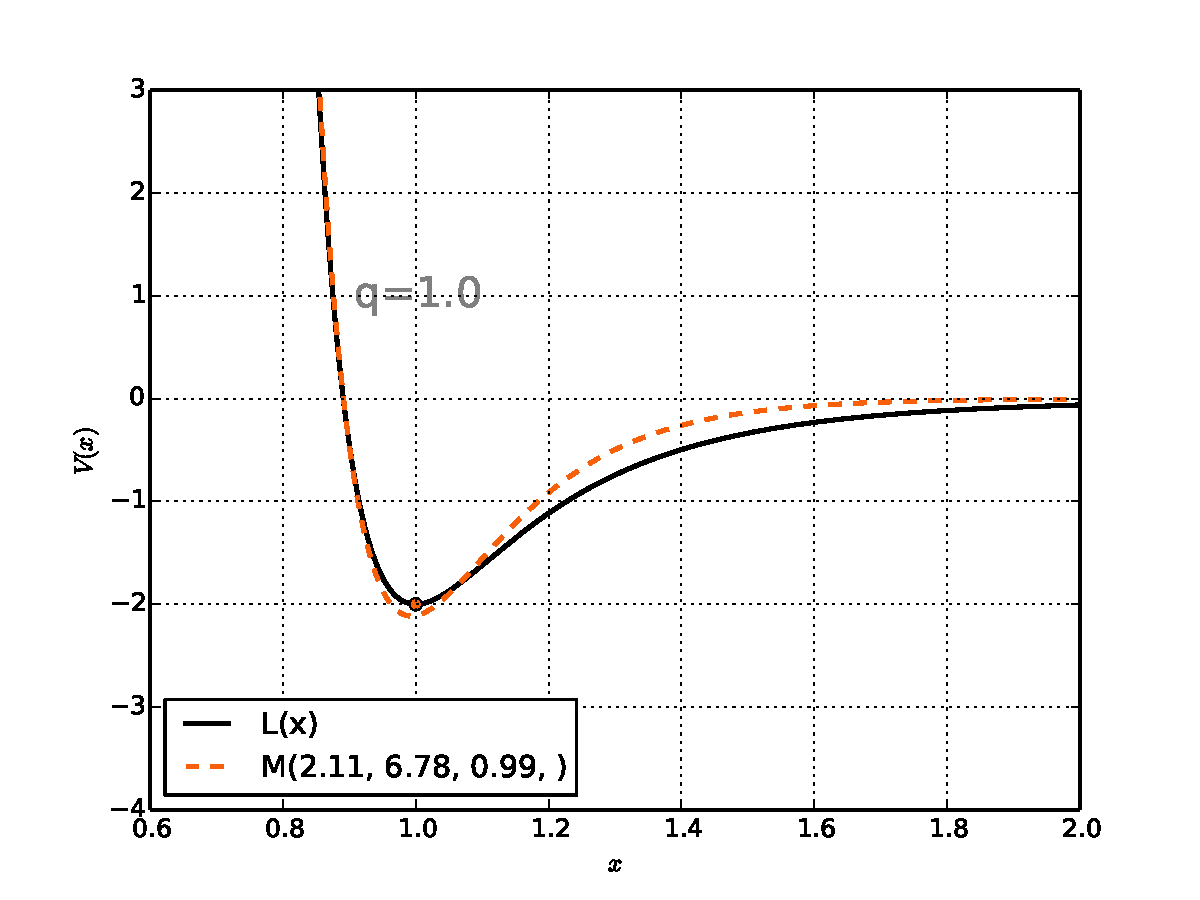
\includegraphics[width=0.5\linewidth]{./figures/MorseFitsLeastsq/leastsq10.pdf}
%    }
%    \\
%     \subfloat[][]{
%	\label{fig:LeastSq11}
%	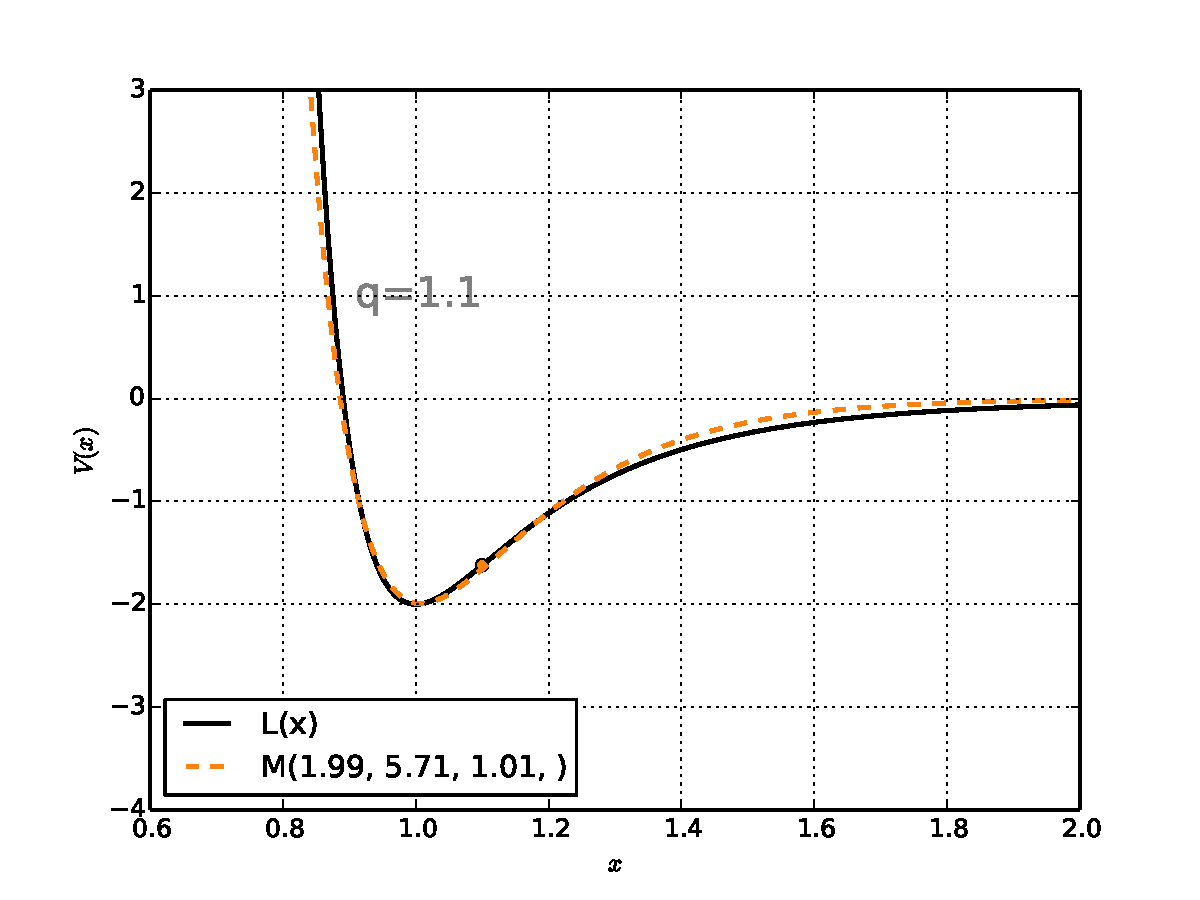
\includegraphics[width=0.5\linewidth]{./figures/MorseFitsLeastsq/leastsq11.pdf}
%    }
%    \subfloat[][]{
%	\label{fig:LeastSq115}
%	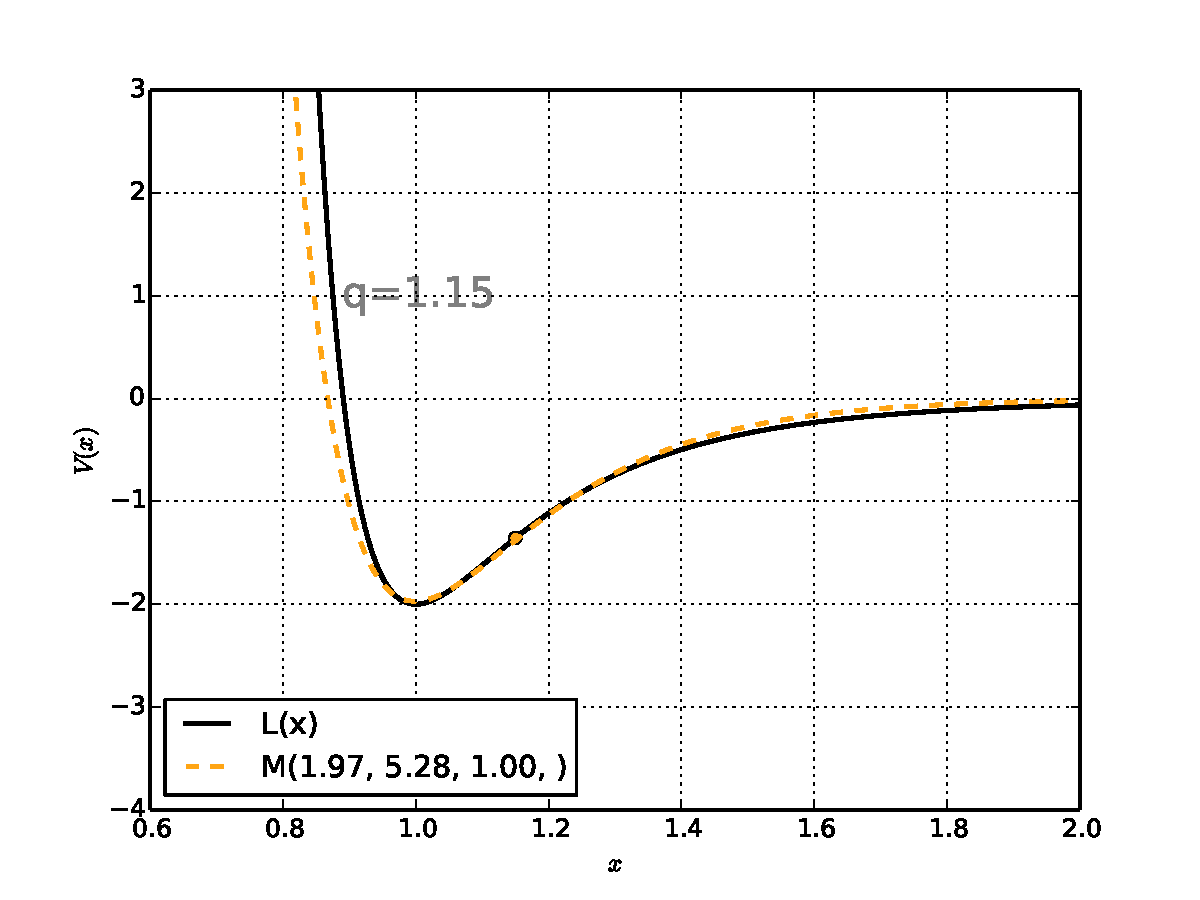
\includegraphics[width=0.5\linewidth]{./figures/MorseFitsLeastsq/leastsq115.pdf}
%    }\\
%    \subfloat[][]{
%	\label{fig:LeastSq12}
%	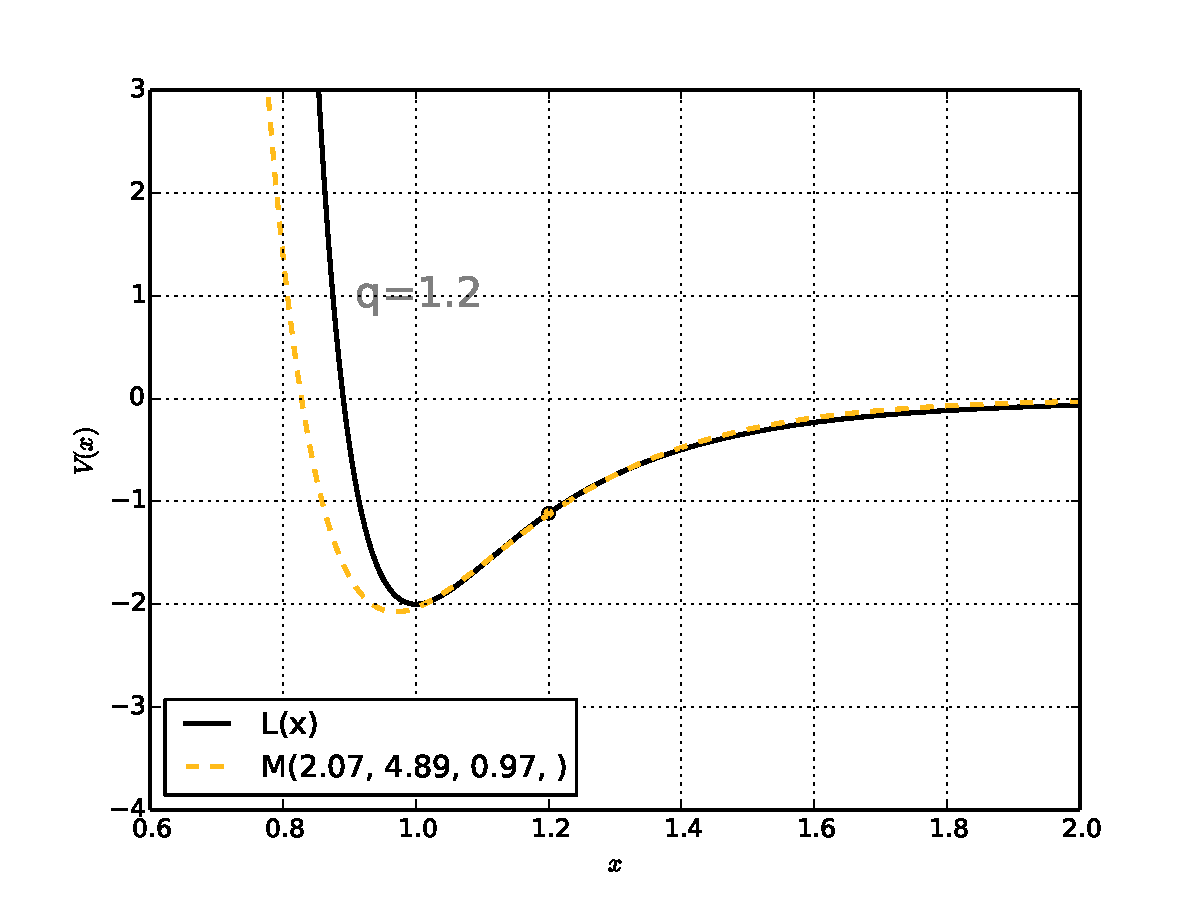
\includegraphics[width=0.5\linewidth]{./figures/MorseFitsLeastsq/leastsq12.pdf}
%    }
%    \subfloat[][]{
%	\label{fig:LeastSq125}
%	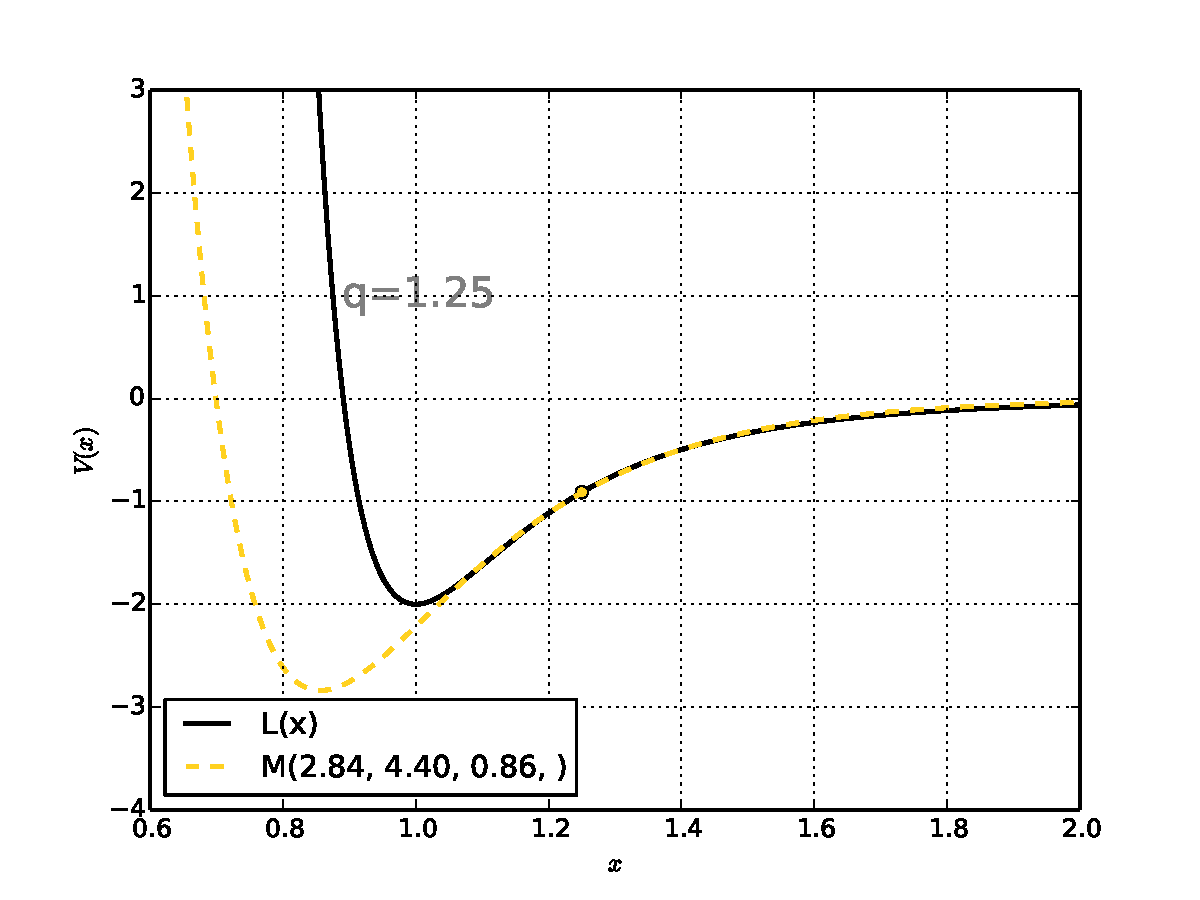
\includegraphics[width=0.5\linewidth]{./figures/MorseFitsLeastsq/leastsq125.pdf}
%    }
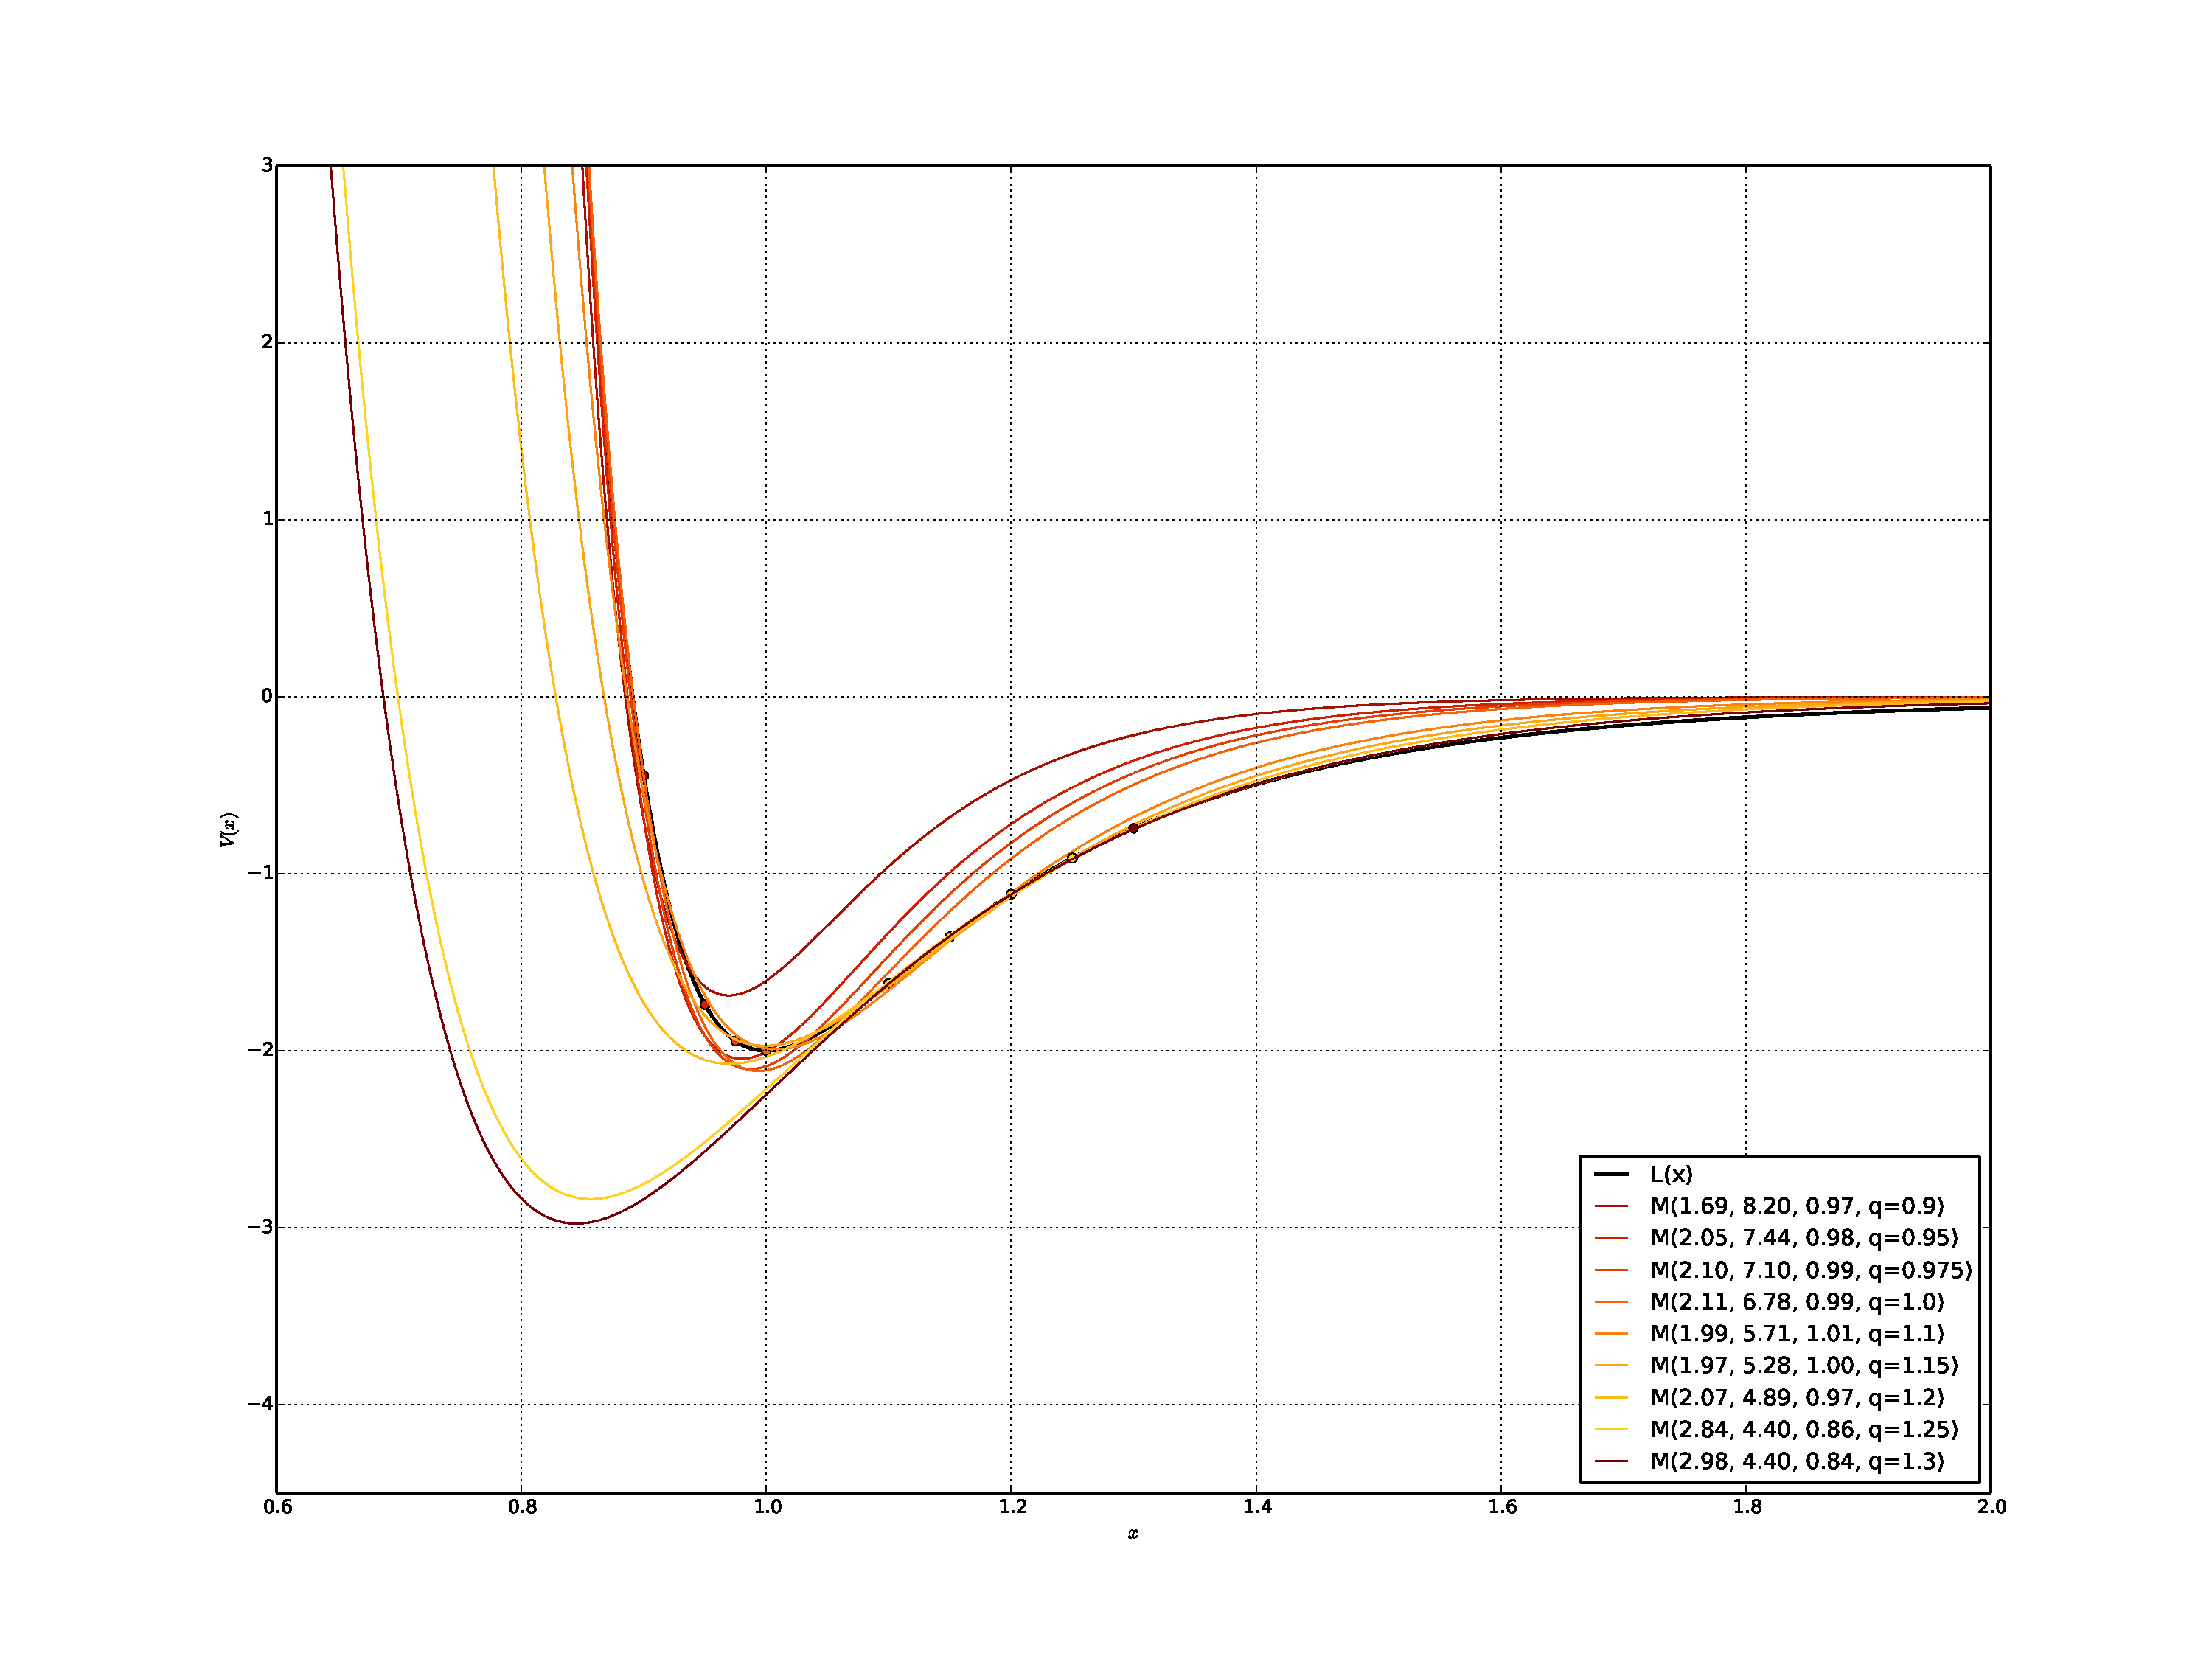
\includegraphics[width=1.2\linewidth]{./figures/MorseFitsLeastsq/leastsqAll.pdf}
    \\
%	\subfloat[][]{
%	\label{fig:LeastSq13}
%	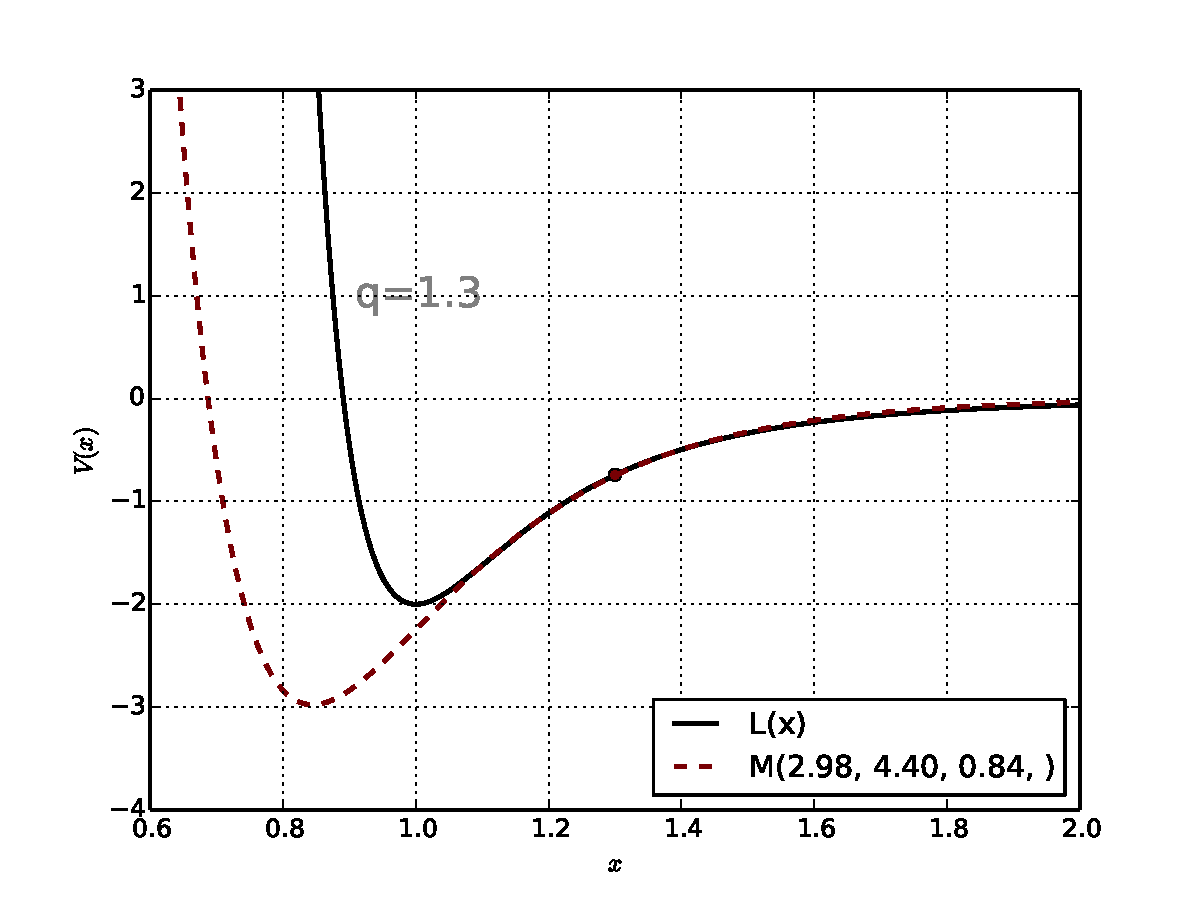
\includegraphics[width=0.5\linewidth]{./figures/MorseFitsLeastsq/leastsq13.pdf}
%    }

       \caption[\texttt{leastsq} fits to the Morse potential]{
	\texttt{leastsq} fits to the Morse potential
    \label{fig:MorseFitsLeastsq}
    }

\end{figure}


%\begin{figure}[h!]
%	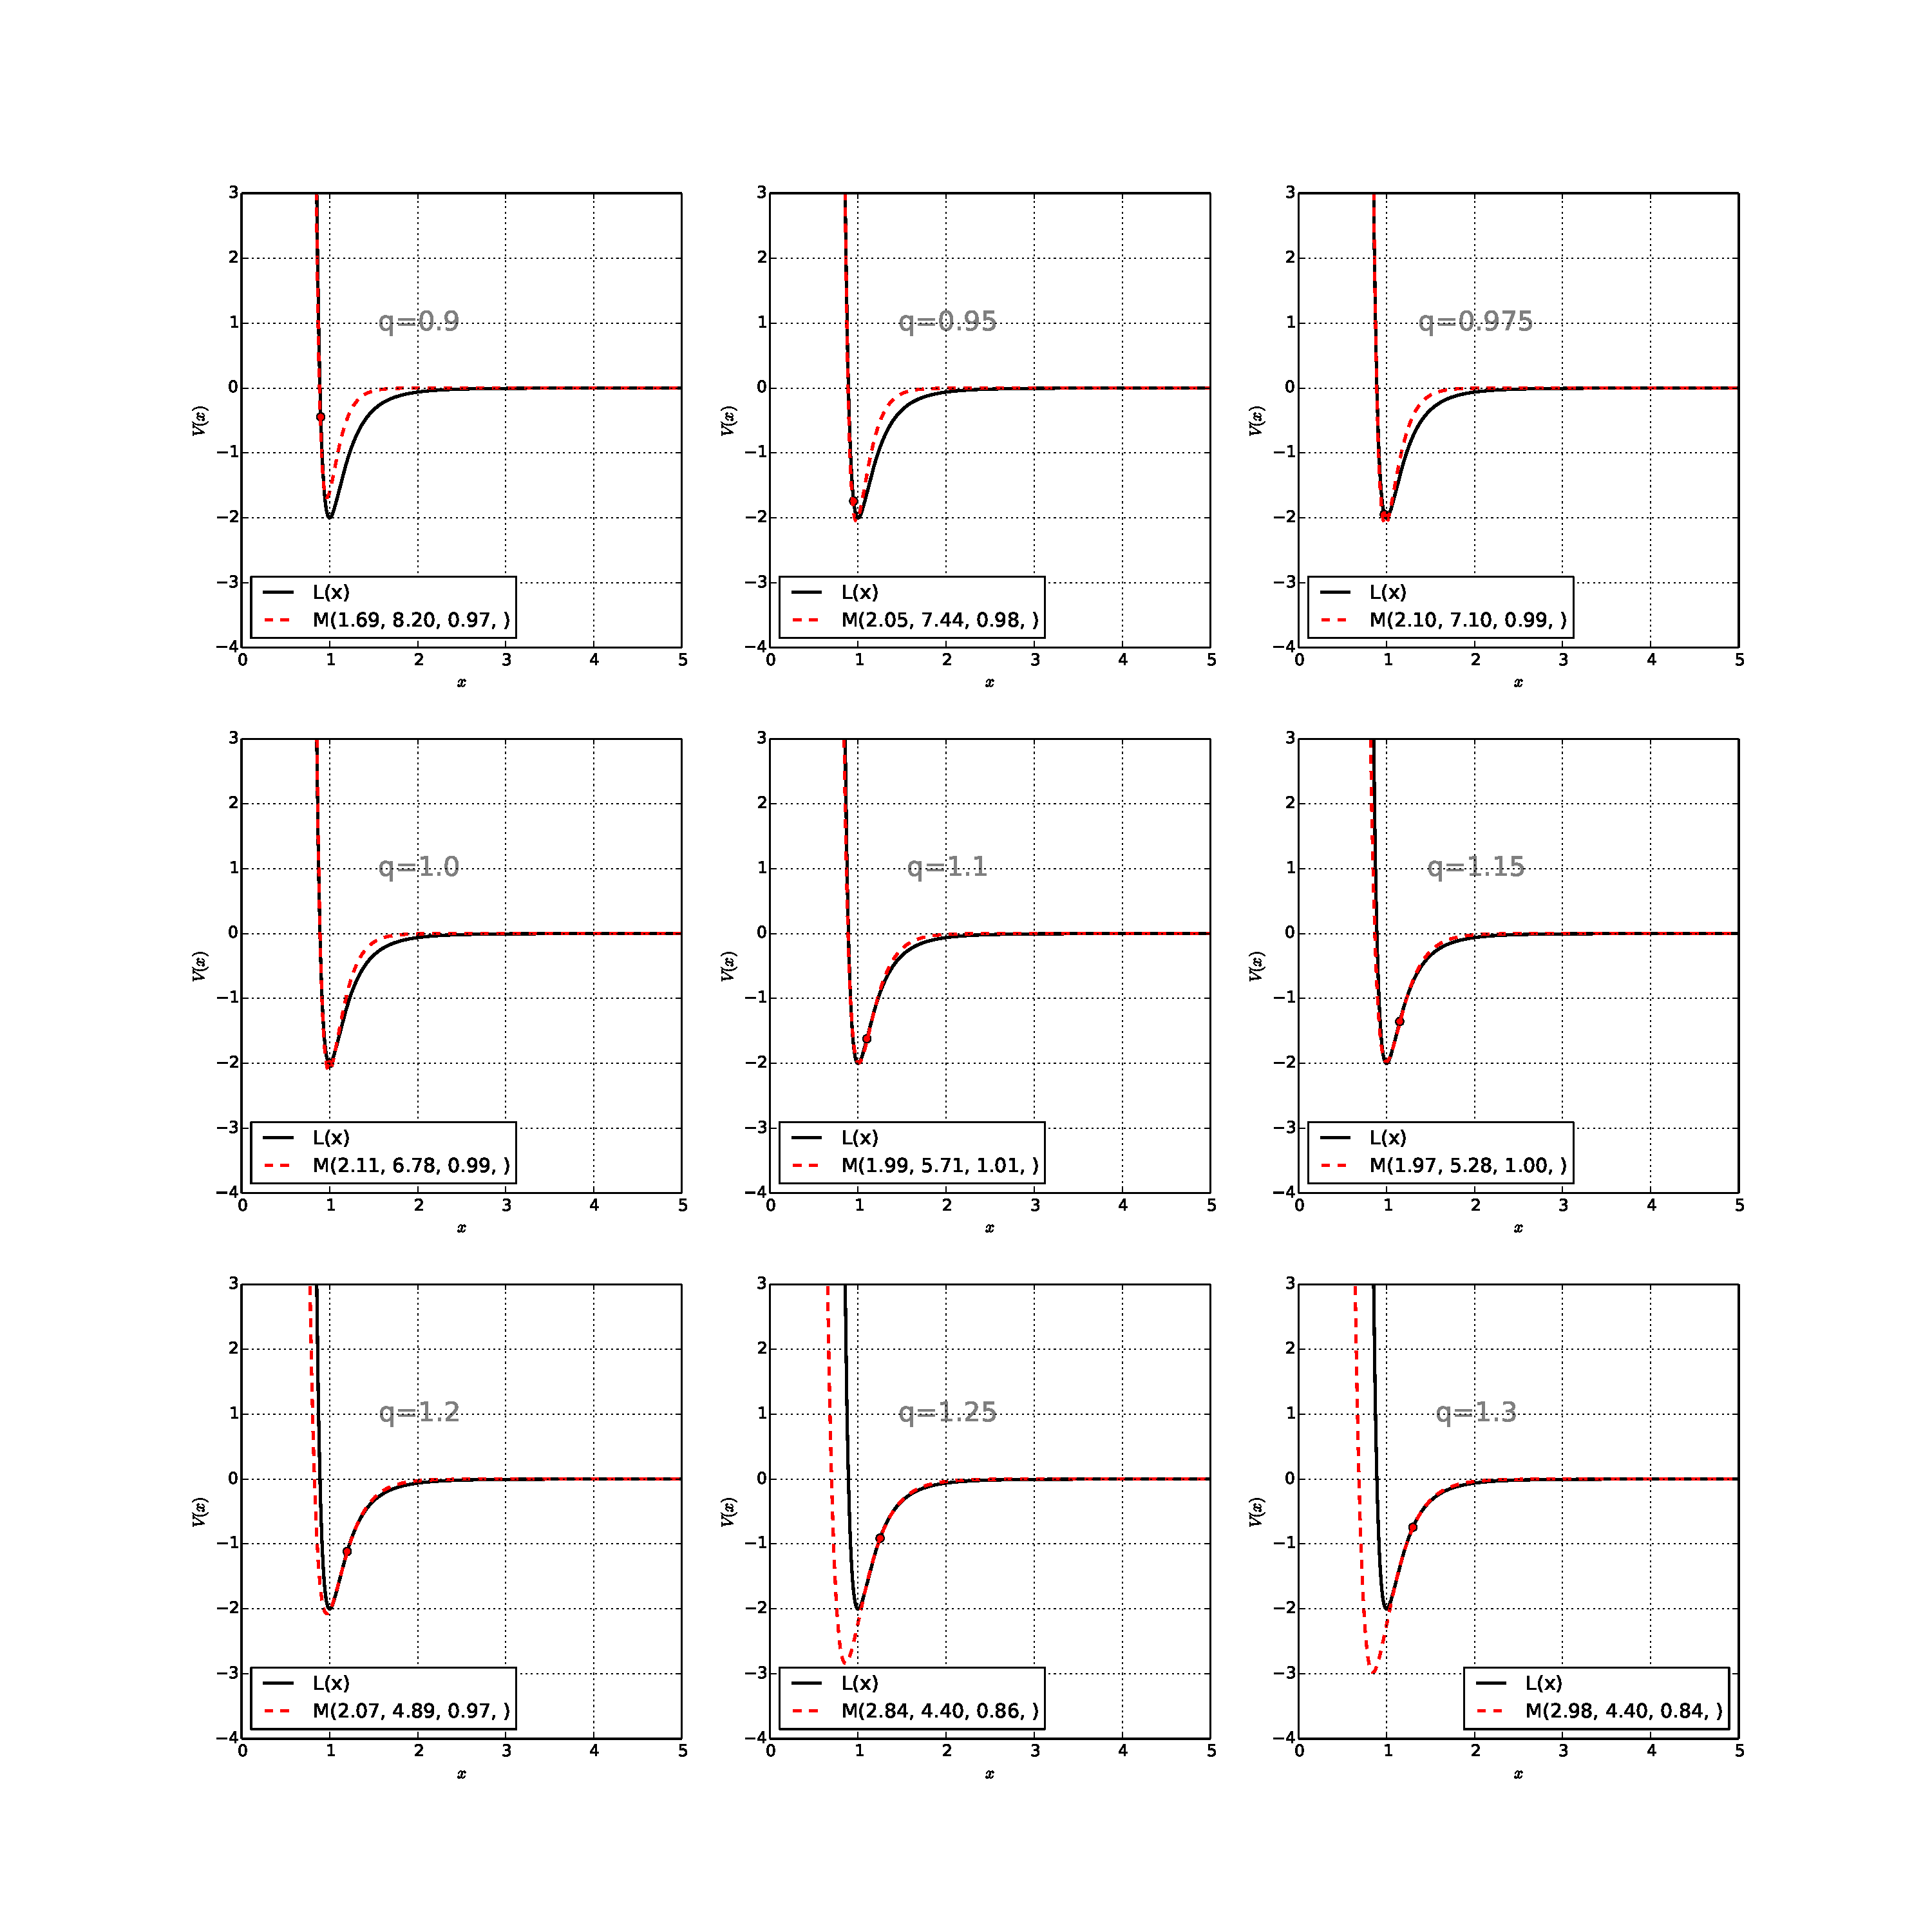
\includegraphics[width=1.0\linewidth]{./figures/MorseFitsLeastsq/fits_leastsq.pdf}
%	\caption[\texttt{leastsq} to the Morse potential]{
%	
%	    \label{fig:MorseFitsLeastsq}
%    }
%
%\end{figure}


\end{chapter}
